\chapter{\label{ch:3-orion}Attosecond X-ray harmonics on the ORION laser facility} 

\minitoc

\section{A plan}

While simulations are relatively cost effective and experiments cumbersome and technically challenging, the proliferation of errors in simulation codes lead to their deviation from reality while reality itself deviates from the idealistic input conditions to the codes. For now, at least, experimentation remains an essential component of the scientific method. Thus, our expectations must also be scaled back to reality. This chapter reports on our March 2023 experiment on the ORION laser facility, AWE, Aldermaston. The UK's most powerful sub-picosecond laser. Yet, one cannot access the ZVP parameter space at these intensities and pulse durations: the $S$ parameter is too large and the preplasma scale length too steep. Instead, this chapter will focus on the ROM model of HHG. 


Have a look at the intro in baeva's thesis, good outline, include first solid HHG observation and oscillating mirror model.

The early developments in the field are outlined by Teubner \textit{et al} \cite{teubnerHighorderHarmonicsLaserirradiated2009}.

%`The first experimental observations of femtosecond high-order harmonics were made independently by Kohlweyer et al. 􏰀1995􏰁 and von der Linde et al. 􏰀1995􏰁'

HHG from solids has demonstrated significantly higher conversion efficiencies than for HHG from gases nor are there any limitations to the applied laser intensity \cite{teubnerHighorderHarmonicsLaserirradiated2009}. SHHG has thus been a field of huge interest over the past three decades for the production of bright coherent attosecond harmonics.



SOme applications
Applications
Bright high harmonics of the laser pulse
Novel bright attosecond duration X-ray diagnostics
%Improved penetration of dense targets  auxiliary heating of ICF targets
%Coherent focusing of high harmonics to their diffraction limit  1000 times intensity gain at focus (Vincenti, PRL, 2019)
Accessing the Schwinger Limit in vacuum
Photon-photon scattering


For CWE: https://iopscience.iop.org/article/10.1088/0953-4075/43/21/213001/pdf
Note that somewhere in this paper they say CWE optimises for 0.02 lambda (use this to explain why in ORION short sim I used a lambda slightly larger than this)


\section{The experiment}
The two experimental goals were to resolve and measure the absolute intensity of X-ray harmonics produced with the ORION SP2 beamline. After debris from the plasma mirror optic damaged the parabola we were required to switch to the higher contrast but lower energy SP1 beamline and only after the experiment did we established it was not possible to resolve X-ray harmonics with the ORION target chamber geometry. However, we were able to measure the absolute intensity for both SP1 and SP2 beamlines and for CVD and PMMA targets.

% TODO move this to appendix or intro
Typical ORION and GEMINI beam paramaters are presented in Table \ref{tab:laser_params}.
\begin{table}[]
	\centering
	\begin{tabular}{lccc}
		\hline \hline
		Parameter                & \multicolumn{2}{c}{ORION} & GEMINI \\ 
		Beamlines                & SP1         & SP2         & N \& S  \\ \hline
		Power (PW)               & 0.5         & 1           & 0.5    \\
		Energy (J)               & 200         & 500         & 12     \\
		Wavelength (nm)          & 527         & 1053        & 800    \\
		Parabola, $f/\#$ & $f/3$        & $f/3$        & $f/2$      \\
		Focal spot FWHM ($\mu$m) & < 20        & < 10        & 2      \\
		Duration (fs)            & 500         & 500         & 40     \\
		Shot rate                & 5/day       & 5/day       & 3/min  \\
		Peak $a_0$ (approx)      & 10          & 30          & 24    \\ \hline \hline
	\end{tabular}
	\caption{The ORION and GEMINI petawatt class short pulse beamlines for comparison. The GEMINI North (N) and South (S) beamlines are equivalent.}
	\label{tab:laser_params}
\end{table}
The GEMINI-PW laser facility of the \ac{CLF} at Harwell Campus, Oxfordshire is a petawatt class facility consisting of two 30 fs beams, \ac{N} and \ac{S}, each delivering a maximum focused intensity of \qty{2e21}{W.cm^{-2}} at a repetition rate of 0.05 Hz. Such high frequency of operation has led to a paradigm shift in high power laser physics experimentation with the arrival of statistically significant results.

The ORION SP1 is produced by passing the SP2 through two frequency doubling crystals creating two equivalent beamlets that are then overlaid at the target. The double beamlet structure at the near-field is imaged in Figure \ref{fig:oriondoublebeamletsnearfield}.
\begin{figure}
	\centering
	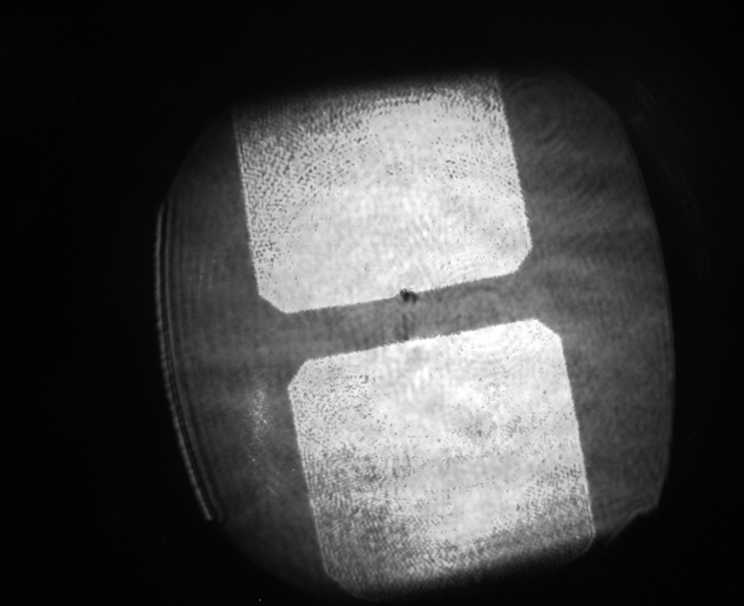
\includegraphics[width=0.5\linewidth]{figures/orion/orion_doublebeamlets_near_field}
	\caption[Image of the ORION SP1 double beamlet structure in the near-field.]{Image of the ORION SP1 double beamlet structure in the near-field. The two beamlets are then superimposed at the target.}
	\label{fig:oriondoublebeamletsnearfield}
\end{figure}

The ORION SP2 beamline intensity temporal profile can be modelled as
\begin{equation}\label{eq:orion_SP2_temporal}
	I_\mathrm{SP2} \sim (I_{0 \ \mathrm{p}}\sech(t/t_\mathrm{p})^2 + I_{0 \ \mathrm{pp}}e^{-(t/t_\mathrm{pp})^2} + I_{0 \ \mathrm{ps}}e^{-\mathrm{abs}(t)/t_\mathrm{ps}} + I_{0 \ \mathrm{ns}}e^{-(t/t_\mathrm{ns})^8}),
\end{equation}
where the constants are detailed in Table \ref{tab:orion_pedestals} \cite{dhillierModelORIONContrast2022}.
\begin{table}[]
	\centering
	\begin{tabular}{lcc}
		\hline\hline
		Pedestal, $i$                & $I_{0 \ i}$ & $t_i$  \\ \hline
		Main pulse, p                & 1           & 0.2 ps \\
		Picosecond pump residual, pp & $10^{-3}$   & 3 ps   \\
		Picosecond pedestal, ps      & \num{5e-5}  & 8 ps   \\
		Nanosecond pedestal, ns      & $10^{-11}$  & 3 ns  \\ \hline \hline
	\end{tabular}
	\caption{The native ORION SP2 pulse and prepulse pedestal constants as defined in Equation \ref{eq:orion_SP2_temporal}.}
	\label{tab:orion_pedestals}
\end{table}
The picosecond pump residual arises from parametric fluorescence in the ps OPA, the picosecond pedestal from scatter in the stretchers and noise on the OPA pump laser and the nanosecond pedestal from parametric fluorescence from the nanosecond OPAs. 
% TODO understand the above.
The SP1 temporal intensity profile is
\begin{equation}
	I_\mathrm{SP1} \sim (I_\mathrm{SP2}^2 + I_\mathrm{SP2} \times 10^{-8}).
\end{equation}
The second term is due to limitations of the harmonic separation system. The frequency doubling mechanism is not 100 \% efficient, \textit{i.e.} some of SP2 beamline remains and must be filtered out. The main pulse of the GEMINI beamlines is more approriately modelled as a Gaussian.
% TODO add a plot of the gemini contrast

The experimental design is relatively straightforward. CAD drawings of the experimental setup are presented in Figure \ref{fig:orioncad}.
\begin{figure}
	\centering
	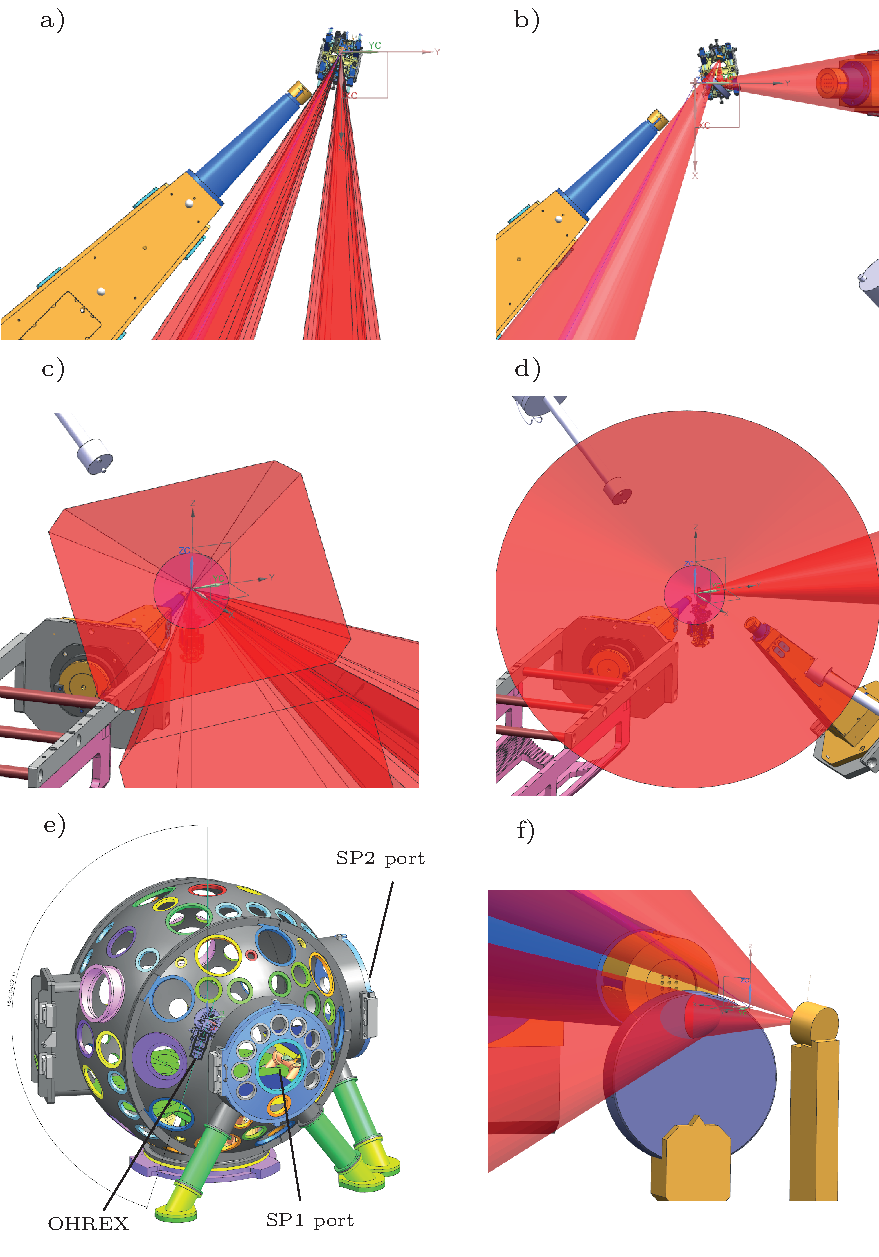
\includegraphics[width=1\linewidth]{figures/orion/orion_cad}
	\caption[ORION HHG experiment target chamber set up.]{\textbf{CAD images of the ORION target chamber set up for this experiment.} a) and b) SP1 and SP2 beamlines respectively from parabola to TCC to OHREX spectrometer. c) and d) SP1 and SP2 beamlines respectively looking from OHREX to TCC. e) Annotated ORION target chamber model. f) SP2 beamline reflecting off plasma mirror before main target incidence.}
	\label{fig:orioncad}
\end{figure}
The laser is focused onto the target at \ac{TCC} with the \ac{OHREX} spectrometer positioned along the specular reflection direction. Additional X-ray pinhole diagnostics monitor the spot size. The SP2 beamline reflects off an additional \ac{PM} optic at \qty{45}{\degree} \ac{AOI} to improve the laser prepulse contrast. Then both the SP1 and SP2 beamlines arrive at \ac{TCC} along the same axis.

Both the non-linear HHG interaction and the linear OHREX crystal spectrometer are sensitive to the polarisation of incident light. It is therefore important to track the polarisations of the beamlines as they propagate through the system.

The ORION target chamber has its own defined geometry with the target located at the origin (\ac{TCC}), described in Figure \ref{fig:miscoriontargetchambergeometry}.
\begin{figure}
	\centering
	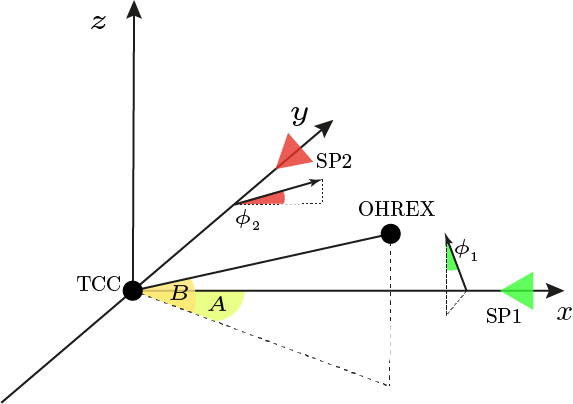
\includegraphics[width=0.7\linewidth]{figures/misc/misc_ORION_target_chamber_geometry}
	\caption[ORION target chamber geometry]{ORION target chamber geometry with the location of the target, OHREX spectrometer and the SP1 (green) and SP2 (infra-red) beamlines and their corresponding polarisations, $\phi_1$ = \qty{11.8}{\degree} and $\phi_2$ = \qty{16.4}{\degree}.}
	\label{fig:miscoriontargetchambergeometry}
\end{figure}
The polarisation angles are $\phi_1 = \qty{11.8}{\degree}$ and $\phi_2 = \qty{16.4}{\degree}$. Following reflection of the SP2 beam off the plasma mirror, both the SP1 and SP2 beamlines propagate in the -$\hat{\mathbf{x}}$-direction  towards the origin. The OHREX crystal is located at 
\begin{equation}
	\mathbf{r}_\mathrm{OHREX} = r_0(\cos B\cos A,-\cos B\sin A, \sin B),
\end{equation}
where $r_0 = \qty{2.4}{m}$, $A = \qty{26.82} {\degree} $ and $B = \qty{18.15}{\degree}$, setting the rotation angle of the target. This was achieved using the ORION Multi-Target-Mounts. Alignment was performed offline by Dr Ed Gumbrell and no further details will be provided here on that process. As in Figure \ref{fig:orioncad}e, the OHREX spectrometer sits on the outside of the target chamber tilted an angle \qty{18}{\degree} to the vertical.

The interaction plane is defined by the vector
\begin{equation}
	\mathbf{n} = \frac{\mathbf{r}_\mathrm{OHREX}}{r_0} \times  \hat{\mathbf{x}} = (0,\sin B, \cos B\sin A).
\end{equation}
The cosine rule can be applied to determine the polarisation of the laser pulses in the interaction plane, for polarisation vector $\hat{\mathbf{E}}$,
\begin{equation}
	\frac{\mathbf{n}}{|\mathbf{n}|}\cdot\hat{\mathbf{E}} = \cos\theta,
\end{equation}
where $\theta$ defines the angle between the polarisation vector and the vector normal to the interaction plane. This corresponds to angles out of the interaction plane of \qty{42.2}{\degree} for the SP1 beam (rotating anticlockwise out of the interaction plane when looking from TCC to parabola) and \qty{19.6}{\degree} for the SP2 beam (rotating clockwise out of the interaction plane when looking from TCC to parabola). Again applying the cosine rule, the angle of incidence is \qty{16}{\degree}.

The polarisation vector can then be split into s- and p-polarised components. The s-polarised component remains unchanged by the interaction but the p-polarised component must be rotated, its direction along $\mathbf{n} \times \mathbf{r}_\mathrm{OHREX}$. In Section \ref{ch:3-sec:simulations}, I show the s-polarisation component is suppressed at the X-ray photon energies of interest and therefore can be neglected.

The OHREX spectrometer sits flat on the target chamber wall but is rotated an angle $C= $ \qty{18}{\degree} to the vertical. The OHREX interation plane is correspondingly rotated. Again, applying the cross-product, the OHREX interaction plane is 
\begin{equation}
	\mathbf{n}_\mathrm{O} = [-\cos(A)\sin(B)\sin(C)-\sin(A)\cos(B)\cos(C),-\cos(A)\cos(B)\cos(C)+\sin(A)\sin(B)\sin(C),\cos(B)\sin(C)].
\end{equation}
Applying the cosine rule between the p-polarised vector and $\mathbf{n}_\mathrm{O}$, the angle of the polarisation vector of the harmonic beam out of the plane of the OHREX interaction is \qty{77.23}{\degree} for both SP1 and SP2.

% TODO Also discuss the fabulous result that generally one can simply extract the results in the Smilei units and multiply by the relevant factors of the frame of interest and thus not worry too much about frame transformations. (add this to bourdier discussion)

% TODO I must redo boosted section since I have made a mistake there and rethink a bit about optimum theta.

% TODO I must also at some point just state that a hat indicates a normalised vector.

%TODO Note that this section needs redoing, there is a new jupyter lab notebook for calculating values in ORION_analysis_sims/experiment_data_analysis on archer2 and called polarisations.ipynb

% TODO READ https://www.nature.com/articles/s42005-024-01575-z
% TODO https://www.nature.com/articles/ncomms12515
\subsection{Targets}
Specialised target holders were designed and built by the AWE and CLF target fabrication teams. These hold the targets at the required angle out of the horizontal plane with an additional fiducial wire for alignment. Targets were mounted on the ORION Multi-Target-Mount and alignment performed offline by Dr Ed Gumbrell.

One might assume that target surface variation, root-mean-square roughness, $\Delta s$, need be less than the highest harmonic order that one wished to generate, however, Dromey \textit{et al} demonstrated categorically in both experiment and simulation that surface roughness need only be less than the excursion amplitude of the oscillating electrons at the target front surface thus ensuring specular reflection and preventing scattering into the wings of the harmonic beam \cite{dromeyDiffractionlimitedPerformanceFocusing2009}. This is generally satisfied by $\Delta s \ll \lambda_\mathrm{L}$. In their experiment, harmonics were visible provided $\Delta s < \lambda_\mathrm{L}/16$. Furthermore, preplasma expansion leads an increase in target smoothness prior to the main pulse arrival.

There are multiple considerations when it comes to target density. Simulations have repeatedly emphasised the improvement of harmonic efficiency for reduced similarity parameter, $S$, \cite{gonoskovUltrarelativisticNanoplasmonicsRoute2011, edwardsXRayEmissionEffectiveness2020} corresponding to low electron density solid targets. In practice accessing the $S\approx 1$ regime is not possible using a petawatt class laser system with even the lowest density solid plastic targets. However, the 2007 Vulcan experiment successfully reproduced the $8/3$ scaling up to the X-ray regime for $S \approx 50 $ \cite{dromeyBrightMultikeVHarmonic2007}. At the same time, as discussed in Section \ref{ch:3-sec:theory}, target hole boring leads to an increased harmonic beam divergence. High electron density targets are perhaps therefore more suited to the petawatt class laser system thereby maintaining beaming of harmonics.
% TODO find that paper where they show that CSE lowers the roll off point, I definitely did read this somewhere...
% Vulcan had CH targets, a0 on target of approx 6.2, normalised density approx 308.
%TODO comment on improvement of S parameter for PMMA leading to an increase in signal strength?

% TODO use the word perturbation for surface roughness
The surface roughness of a selection of low density plastic targets were analysed by the CLF target fabrication team leading to the choice of PMMA plastic targets. CVD targets were also selected, having the highest ionisation potential (and therefore lowest susceptibility to laser prepulse) of solids that can be polished optically flat albeit at a higher $S$ parameter. Scans performed by AWE and CLF of the target surfaces are given in Figure \ref{fig:oriontargets}.
% TODO add this back in, its annoying me currently by disappearing
\begin{figure}
	\centering
	%\includegraphics{figures/orion/orion_targets}
	\caption[ORION HHG experiment targets]{\textbf{ORION experiment 3D scans of target roughness.} a) CVD with roughness $\Delta s$ = \qty{4}{nm} and $S \approx$ 26, 35 for SP1 and SP2 beamlines respectively. b) PMMA with roughness $\Delta s$ = \qty{11.2}{nm} and $S \approx$ 10, 13 for SP1 and SP2 beamlines respectively.}
	\label{fig:oriontargets}
\end{figure}
% TODO confirm I can include the PMMA scan from TFAB

\subsection{Contrast and plasma mirrors}
As illustrated in Figure \ref{fig:orioncad}, a plasma mirror optic is included before the main target to improve the contrast of the SP2 beamline \cite{doumyCompleteCharacterizationPlasma2004}. HYADES simulations of the effect of this optic are detailed in Section \ref{sec:orion-hydro}. The distance between the PM and the main target is \qty{15}{mm}, thus the beam diameter at the PM is $\approx 15/(f/3) = \qty{5}{mm}$ and the intensity on PM can be calculated. Provided the harmonic beam divergence is less than or equal to the $f/3$ cone, as is anticipated, the harmonic beam should not be clipped by the PM in this setup. 
%TODO calculate that intensity and show it is where it should be.

The intention was to use \ac{AR}-coated fused silica optimised for \qty{45}{\degree} \ac{AOI} and the SP2 pulse wavelength (BCP45R) \cite{45AOIBeamsplitter}. This has a reflectance of \qty{0.398}{\%} at $\lambda_\mathrm{L} = \qty{1053}{nm}$ for unpolarised light. Unfortunately the debris from the PM caused damage to the parabola. For the second SP2 shot, the high reflectivity fused silica PM was replaced with a thin foil of silicon nitride. The reduction in available material of the thin foil reducing the risk of damaging debris. At \qty{45}{\degree} \ac{AOI}, $\lambda = \qty{1.053}{\mu m}$ and $\phi_2 = \qty{16.4}{\degree}$, the silicon nitride PM pre-switch-on has a reflectivity of \qty{5.55}{\%} \cite{polyanskiyRefractiveindexInfoDatabase2024}. One can assume its behaviour after switch-on is consistent with the other PM since it is simply a plasma interaction now.
%TODO intro section on laser contrast included function of DPM

\subsection{KBRXM}
The ORION SP1 and SP2 spot size was routinely monitored on shot by the AWE laser team via two X-ray pinhole cameras and the time-integrating Kirkpatrick-Baez X-ray microscope (KBXRM) diagnostic, sat on the target chamber Port 21 and pointed at the notional \ac{TCC}. This reflective X-ray microscope optic has a ten times magnification and spatial resolution of \qty{15}{\mu m}, comfortably resolving the laser spot size. Images were again recorded with TR-type IP. While direct mapping between the recorded images and real laser irradiance profiles is a highly non-trivial problem with any proposed model depending strongly on the assumptions made. However, by making the very reasonable assumption of spatial and temporal blurring of the spot size in the X-ray image due to electron transport away from the laser spot, clearly the measured spot size will be an upper bound on the real spot size. It follows that the upper bound on optical spot widths corresponds to a lower limit of irradiance (since the on shot energy is well-defined). These diagnostics determine sensible upper bounds for the laser spot size are \qty{20}{\mu m} and \qty{10}{\mu m} for the SP1 and SP2 beamlines respectively.

\section{\label{ch:3-sec:theory}Theory}
Note: in the below all we are simply saying is the reflected field is simply the negative of the incoming field with a phase modulation \cite{derbruggeEnhancedRelativisticHarmonics2010}. See also this paper for a simle explanation of OMM

For the moderately relativistic sub-picosecond ORION SP1 and SP2 beamlines the most appropriate description of their non-linear interaction with a solid density target is the Relativistic Oscillating Mirror (ROM) model. The full mathematical formation of which forms the main body of Baeva's 2008 thesis \cite{baevaHighHarmonicGeneration2008}, a notably more rigorous derivation than her original paper on the same topic \cite{baevaTheoryHighorderHarmonic2006}, applying the highly general Apparent Reflection Point formulism to the case of $S>1$ in relativistic similarity theory, showing that it coincides with the motion of the relativistic critical density surface. The following covers the more qualitative, physically motivated understanding of why this theory works, which is fundamentally that while the surface motion is generally complex and parameter space dependent, at the important point the surface motion is always parabolic. By application of the Bourdier method, Baeva demonstrated that the envelope of the spectral content of the reflected beam does not deviate from the normal incidence linearly polarised case for either s- or p-polarised incidence. Thus the following discussion will be restricted to normal incidence. One starts with relativistic similarity theory and Equation \ref{{eq:intro-p_similarity}}, $\mathbf{p} \sim a_0$. As discussed in Section \ref{sec:zvp-intro}, microscopically electrons follow similar relativistic trajectories yet from Equation \ref{eq:zvp-vprop}, $v_\mathrm{prop}$, the velocity of electrons along the propagation axis of the laser pulse, not necessarily relativistic except at the passing of the zero of the vector potential where $v_\mathrm{prop} \to c$. Macroscopically, the well-defined critical density surface within the skin depth (located at $S =1$), has a gamma factor that tracks the electrons' velocity along the propagation direction ($x$-direction) at that point,
\begin{equation}\label{eq:orion-gamma_s}
	\gamma_\mathrm{s} = \frac{1}{\sqrt{1-v_\mathrm{prop}^2/c^2}} = \sqrt{ \frac{1 + a(t,x)^2 +  p_\mathrm{prop}^2/(m_\mathrm{e}c)^2}{1 + a(t,x)^2}}.
\end{equation}
Equation \ref{eq:orion-gamma_s} indicates surface gamma factors of order unity except at zeros in the vector potential at which point $\gamma_\mathrm{s} \sim a_0$. In the viscinity of the zero, $a \sim a_0\sin(\omega_L t) \approx a_0\omega_\mathrm{L}t$. Thus, while the velocity of the surface is a smoothly varying function around the maximum, $v_\mathrm{s,\, max} \sim 1 - \mathcal{O}(a_0^{-2})$, the \textit{gamma factor spikes} as the vector potential passes through zero and it is at this point that the surface emits high frequency photons. One can then approximate the duration of this high frequency component of the pulse. The surface will begin radiating such photons at some point near the gamma spike and continue radiating until the gamma factor drops down again after the gamma spike. In ZVP we observe the zero overtaking the emitted photons and thus radiation from the extended electron bunch that is emitted first arrives at the observer last. Here, we consider one point in the sub-light speed surface emitting radiation, thus the radiation overtakes the surface and points emitted first are observed first. The radiation emitted therefore has a duration of
\begin{equation}
	\Delta l \approx (c-|\mathbf{v}_\mathrm{s,\, max}|)\Delta t \approx \frac{\Delta t}{\gamma_\mathrm{s,\, max}^2},
\end{equation}
where $\Delta t$ is the temporal duration of the gamma spike. 

Writing the surface velocity as a smooth function around its maximum,
\begin{equation}\label{eq:orion-vs}
	\mathbf{v}_\mathrm{s}(t) = -(v_\mathrm{s,\, max} - c\alpha(\omega_\mathrm{L}t)^2) \mathbf{\hat{x}}.
\end{equation}
Without loss of generality the peak of the gamma spike is set to $t=0$ for cleaner notation. Around the gamma spike, the surface gamma factor is thus
\begin{equation}
	\gamma_\mathrm{s}(t) \approx \frac{1}{\sqrt{1-(\mathbf{v}_\mathrm{s,\, max}/c)^2 - 2\alpha(\omega_\mathrm{L}t)^2}}.
\end{equation}
Since $1-(\mathbf{v}_\mathrm{s,\, max}/c)^2 = 1/\gamma_\mathrm{s,\, max}^2$, one can calculate the FWHM of the gamma spike is
\begin{equation}
	\Delta t \sim \frac{1}{\sqrt{\alpha }\omega_\mathrm{L} \gamma_\mathrm{s,\, max}}.
\end{equation}
%TODO change this from looking at the FWHM to an arbitrary change in gamma
Hence, $\Delta t_\mathrm{FWHM} \sim a_0^{-1}$ and $\Delta l \sim 1/a_0^{-3}$ and the cut off frequency corresponding to the highest frequency accesible for a pulse of that duration is
\begin{equation}\label{eq:orion-omegac}
	\frac{\omega_\mathrm{c}}{\omega_\mathrm{L}} \sim \sqrt{\alpha}\gamma_\mathrm{s,\, max}^3 \sim a_0^3.
\end{equation}
Within the ROM model these high frequency pulses are coherently produced with the low order harmonics and at intensities that require filtration to access the possible attosecond duration of these pulses.

One can access the harmonic spectrum envelope for lower energies than the harmonic cut off. From the Leontovich boundary conditions
% TODO cite this and add it,
corresponding to zero energy flux at the reflection point.
This corresponds to a balance of the electric fields at the plasma surface, $x_\mathrm{s}$, hence for the incoming and reflected waves,
\begin{equation}\label{eq:orion-Ei_Er}
	E_\mathrm{i}(x_\mathrm{s}(t) - ct) = - E_\mathrm{r}(x_\mathrm{s}(t) + ct)
\end{equation}
for all $t$. Since we are making the approximation of a plane wave, the phase structure at the reflection point will be maintained as the reflected wave propagates away from the interaction region to our observation point ($E_\mathrm{r}(x_\mathrm{s}(t) - ct) = E_\mathrm{r}(x' - ct')$ for an obesrvation point $(x',t')$ near an electric field peak.). Thus, determining the modulation of the reflected beam is akin to solving Equation \ref{eq:orion-Ei_Er}. Writing $\Phi = x_\mathrm{s}(t) - ct$, $\Psi = x_\mathrm{s}(t) + ct$ and taking the time derivative of Equation \ref{{eq:orion-Ei_Er}},
\begin{equation}
	\frac{\mathrm{d}E_\mathrm{r}(\Psi)}{\mathrm{d}\Psi} = \frac{c - \mathbf{v}_\mathrm{s}(t)}{c+\mathbf{v}_\mathrm{s}(t)}\frac{\mathrm{d}E_\mathrm{i}(\Phi)}{\mathrm{d}\Phi}
\end{equation}
where $v_\mathrm{s}(t)$ is given in Equation \ref{eq:orion-vs}. Integrating Equation \ref{eq:orion-vs} the reflected wave phase is
\begin{equation}
	\Psi(t) = \Psi(0) + \frac{ct}{\gamma_\mathrm{s,\, max}^2} + \frac{1}{3}c\alpha \omega_\mathrm{L}t^3.
\end{equation}
Very close to the gamma spike peak the linear term will dominate the interaction, corresponding to the highest order harmonics as discussed previously. The non-linear term dominates for 
\begin{equation}\label{eq:orion-deltaphi}
	\delta \Psi = |\Psi(t) - \Psi(0)| \gg \left(\frac{3}{\alpha}\right)^{1/2}\frac{c}{\omega_\mathrm{L}\gamma_\mathrm{s,\, max}^3}.
\end{equation}
Note the correspondence between Equation \ref{eq:orion-omegac} and the right hand side of Equation \ref{eq:orion-deltaphi}. In this regime we can write
\begin{equation}
	t = \left(\frac{3\delta \Psi }{c\alpha \omega_\mathrm{L}}\right)^{1/3}
\end{equation}

For these intermediate times around the gamma spike the linear term can be neglected, this is equivalent to writing $v_\mathrm{s,\, max} = c$. Thus,
\begin{equation}
	\frac{\mathrm{d}E_\mathrm{r}(\Psi)}{\mathrm{d}\Psi} = \left(\frac{2c - c\alpha (\omega_\mathrm{L}t)^2}{c\alpha (\omega_\mathrm{L}t)^2}\right)\frac{\mathrm{d}E_\mathrm{i}(\Phi)}{\mathrm{d}\Phi}
\end{equation}
We assume the incoming radiation is slowly varying around the short duration of the gamma spike, $\mathrm{d}E_\mathrm{i}(\Phi)/\mathrm{d}\Phi \approx \mathrm{d}E_\mathrm{i}(\Phi)/\mathrm{d}\Phi|_{\Phi = \Phi(0)}$ and so we arrive at an equation we can integrate,
\begin{equation}
	\frac{\mathrm{d}E_\mathrm{r}(\Psi)}{\mathrm{d}(\delta \Psi)} = \frac{2}{\alpha^{1/3}} \left(\frac{c}{3\omega_\mathrm{L}^2 \delta \Psi}\right)^{2/3}\frac{\mathrm{d}E_\mathrm{i}(\Phi)}{\mathrm{d}\Phi}|_{\Phi = \Phi(0)}
\end{equation}
obtaining
\begin{equation}
	E_\mathrm{r}(\Psi) = -E_\mathrm{i}(\Phi(0)) - \left(\frac{3c^2}{\alpha \omega_\mathrm{L}^2}\right)^{1/3}\frac{\mathrm{d}E_\mathrm{i}(\Phi)}{\mathrm{d}\Phi}|_{\Phi = \Phi(0)} \times (\delta \Psi)^{1/3}.
\end{equation}
One can the see therefore that the reflected radiation gets the quasi-singularity
\begin{equation}
	E_\mathrm{r}(x,t) = \mathrm{const}_1 - \mathrm{const_2}\times (ct - x)^{1/3}.
\end{equation}
Consequently, the harmonic content follows the envelope obtained by the Fourier transform,
\begin{equation}
	|E(\omega)|^2 \sim \left|\int (ct-x)^{1/3}e^{-i\omega t} \mathrm{d} t\right|^2 \sim \frac{1}{\omega^{8/3}}.
\end{equation}

% TODO add in the full baeva expressions and discuss.
% TODO note about in ROM the zero propagates at c thus no advance time bunch width.
% TODO approximate pulse duration of filtered pulse and compare it to the theory.
% TODO add a note to say this is envelope and we note that to get the periodicity we need haromics of hte thickess of the incoming laser pulse.
Explain that since we are in the 1D model, Er does not evolve from where it starts at the surface.
\subsection{The ROM model}
% TODO Bourdier methodology in introduction

Apply Bourdier method and conservation of generalised momentum, we see that 

and thus non-linearity

and thus the thing we need to solve is blah.


The laser pulse leads to macroscopic oscillation of the plasma surface and therefore a corresponding oscillation of the ARP. One can understand this leading to a sub cycle Doppler shift in the reflected pulse. These pulses of radiation separated by the laser pulse frequency must therfore in the spectral domain consist of HH.

The \ac{ROM} model describes an extension. 

The following outlines the key ideas 

Ok: assume I have the expression from Baeva's paper (do this tomorrow)

\subsection{The normalisation factor}
Baeva's theory provides us with the relative intensity of harmonics. However, for comparison with the absolute spectral intensity of harmonics in experiment, the normalisation factor is required. This can be calculated from conservation of energy. For arbitrary harmonic order scaling, $n^{-p}$, the spectral intensity of the harmonic beam is
\begin{equation}
	I_\omega(\omega) = \frac{dE_\omega(J)}{dAd\omega} = I_0 \sum^{n_\mathrm{C}}_{n = 1,\ \mathrm{odd}} n^{-p} S_n\left( \frac{\omega}{\omega_\mathrm{L}}-n\right)
\end{equation}
up to the cutoff, $n_\mathrm{C}$. Here $S_n(\omega/\omega_\mathrm{L}-n)$ is the spectral shape function of the $n^\mathrm{th}$ harmonic in reciprocal space and $I_0$ is the normalisation factor of interest. From conservation of energy,
\begin{equation}
	\int I_\omega(\omega) \mathrm{d}\omega \mathrm{d} A = ER,
\end{equation}
% TODO Simulation showing long pulse vs short pulse spectral shape functions relative sizes
where $E$ the total energy of the laser pulse and $R$ is the reflectivity of the \ac{RPM}. Intuition suggests the spectral shape function for the $n^\mathrm{th}$ harmonic retains the spectral shape of the incident laser pulse, \textit{i.e.} for a laser pulse with a Gaussian temporal profile, this corresponds to a Gaussian centred at $n\omega_\mathrm{L}$ of width $\sigma_\mathrm{L} = 1/t_\mathrm{L}$, where $t_\mathrm{L}$ is the laser pulse width. Simulations show this is a reasonable approximation for ORION parameters \footnote{Hole boring discussed in the following section can lead to a Doppler shift in harmonic energy across the laser pulse corresponding to a Doppler broadening of the spectral shape function in reciprocal space, however, unlike the ZVP simulations of the previous chapter, this is negligible for ORION parameters.}.

Simulations also show that for the SP1 laser, the incident laser pulse significantly suppresses the even harmonics, hence,
\begin{equation}
	ER = \int^\infty_0 I_0 \sum^{n_\mathrm{C}}_{n=1,\ \mathrm{odd}}n^{-p}e^{-(\omega/\omega_\mathrm{L} - n)^2/\sigma^2_\mathrm{L}}\mathrm{d}\omega.
\end{equation}
The integral and summation order can be reversed. Since $\sigma_\mathrm{L} \ll \omega_\mathrm{L}$, all integrals in the summation are $\approx \int^\infty_{-\infty}$ and therefore,
\begin{equation}
	ER \approx I_0 \sum^{n_\mathrm{C}/2-1}_{m=0} (1+2m)^{-p} \sqrt{\pi}\sigma_\mathrm{L}\omega_\mathrm{L},
\end{equation}
thus,
\begin{equation}
	ER \approx I_0 \sqrt{\pi}\sigma_\mathrm{L}\omega_\mathrm{L} ((1-2^{-p})\zeta(p) - 2^{-p}\zeta(p,\frac{n_\mathrm{C} + 1}{2})),
\end{equation}
where $\zeta(p)$ and $\zeta(p,(n_\mathrm{C} + 1)/2)$ are the Riemann Zeta and Hurwitz Zeta functions respectively. The final term can be neglected for a petawatt class laser pulse where $n_\mathrm{C} \gg 1$. In the case of an ideal $p$-polarised laser pulse,
\begin{equation}
	ER \approx I_0 \sqrt{\pi}\sigma_\mathrm{L} \omega_\mathrm{L}\zeta(p).
\end{equation}
For the \ac{ROM} regime, $p = 8/3$ and the \ac{RPM} is extremely efficient, $R \approx 1$. Thus, $I_0$ can be estimated from the system parameters.

\subsection{Hole boring}
% TODO add reference to ZVP plots demonstrating hole boring.
As observed in the ZVP plots, on long timescales relative to the laser pulse cycles, via the ponderomotive pressure of the laser, the plasma front moves inwards. This is hole boring \cite{wilksAbsorptionUltraIntenseLaser1992}. One can derive a hole boring velocity by considering conservation of momentum in this quasi-static state. Since the hole boring velocity is laser pulse intensity dependent, the spatial profile of the laser will be imprinted on the surface. Typically Gaussian in shape, for high power laser systems, this can to first order generate a focusing \ac{RPM} and a beaming of the specularly reflected signal, as in Figure \ref{fig:orionholeboring}.
\begin{figure}
	\centering
	\includegraphics[width=0.9\linewidth]{figures/orion/orion_hole_boring}
	\caption[2D PIC simulation of HHG beaming effect via hole boring.]{Electromagnetic field intensity in a 2D PIC simulation of a relativistic ($a_0 = 30$) laser pulse incident on a solid density plasma. The incoming beam is specularly reflected off the target which is curved by the radiation pressure leading to beaming in the reflected harmonic beam.}
	\label{fig:orionholeboring}
\end{figure}
To access the highest possible electromagnetic field intensities, the laser pulse is focused on target to the diffraction limit. However, since the diffraction limit scales linearly with the wavelength, higher-order harmonics can be refocused to a smaller spot via this mechanism allowing access to unprecedented peak intensities. Vincenti \textit{et al} demonstrated intensity gains of over 1000 with currently accessible parameters in \ac{3D} \ac{PIC} simulations \cite{vincentiAchievingExtremeLight2019}, suggesting a realistic route to the Schwinger Limit using next-generation laser facilities. Regardless of any blue-skies purposes, it is clear any prediction of \ac{HHG} beam intensity must account for hole boring and is therefore an essential component of the ORION experiment analysis.

% TODO I might want to flesh out the hole boring analysis but it already takes up so much space so idk...
Applying momentum balance between the laser pulse and particles in the rest frame of the \ac{RPM} surface, the hole boring velocity is
\begin{equation}\label{eq:v_HB}
	\frac{v_\mathrm{HB}}{c} = \sqrt{\frac{R\cos\theta}{2}\frac{Zm_\mathrm{e}}{Am_\mathrm{p}}\frac{n_\mathrm{c}}{n_\mathrm{e}(x_\mathrm{i}(t,y))}}a_L(t,y) = \Pi a_L(t,y),
\end{equation}
where $R$ is the RPM reflectivity, $\theta$ is the angle of incidence, \qty{16}{\degree} in the ORION experiment, $Z$ and $A$ are the atomic and atomic mass numbers respectively for the plasma ions, $n_\mathrm{c}$ is the plasma critical density, $n_\mathrm{e}(x_\mathrm{i}(t,y))$ the electron number density and $x_\mathrm{i}(t,y)$
the depth of hole boring, from the Supplementary Material \cite{vincentiOpticalPropertiesRelativistic2014}. For the ORION laser pulse parameter space $\Pi \ll a_\mathrm{L}\forall t$ , \textit{i.e.} we are in the relativistic electron and non-relativistic ion regime. Hence, the relativistic correction derived by Robinson \textit{et al} \cite{robinsonRelativisticallyCorrectHoleboring2009} to Equation \ref{eq:v_HB} can be neglected. Due to the high contrast and long duration of the ORION beamlines, there is minimal pre-plasma formation on the front surface and therefore the number density is simply the number density of the material in solid form and $n_\mathrm{e}$ is independent of $x_\mathrm{i}(t,y)$. Robinson \textit{et al} \cite{robinsonHoleboringRadiationPressure2009} generalised momentum conservation to multiple species, simply replace the mass density with the composite mass density $\rho = \sum_j m_{\mathrm{i}j}n_{\mathrm{i}j}$, then
\begin{equation}
	\frac{An_\mathrm{e}}{Z} \to \sum_j \frac{A_jn_{\mathrm{e}j}}{Z_j},
\end{equation}
where $n_{\mathrm{e}j}$ is the number density of electrons that originated from the $j$ ion.


%TODO (This analysis can be done by taking the Vincenti 2014 derivation and taking $R =1$, since that applied to ORION parameter space, replace ion terms with sums over ions and make the important assumption: all ions reflected at the same velocity (reasonable), note that this might be a tricky to do to electrons when there is significant electron heating and so $R < 1$, may need to return to this for thesis... manipulating the expression arrives at the desired form)

The spatio-temporal envelope of the normalised vector potential of the laser pulse incident on the target surface is modelled as
\begin{equation}
	a_\mathrm{L}(t,y) = a_0e^{-\frac{y^2}{2w_\mathrm{L}^2}}g(t-t_0)
\end{equation}
where $w_\mathrm{L}$ is the beam waist on target and $g(t)$ the temporal envelope, a Gaussian or $\sech$ profile and $t_0$ the main pulse peak time.

Integrating Equation \ref{eq:v_HB},
\begin{equation}\label{eq:xi_t}
	x_\mathrm{i}(y) = \int v_\mathrm{HB}\mathrm{d}t = \Pi \int^t_{-\infty} a_L(t,y)c\mathrm{d}t.
\end{equation}

At the peak of the main pulse,
\begin{equation}
	x_\mathrm{i}(y) = \Pi a_0ce^{-\frac{y^2}{2w_L^2}} G,
\end{equation}
where $G = \int_\infty^{t_0} g(t-t_0) \mathrm{d} t \sim t_\mathrm{L}$ and $t_\mathrm{L}$ is the laser pulse temporal width.

The total denting is a combination of the peak electron-ion charge separation, $x_\mathrm{e}$ (which leads to the intrinsic phase of the HHG beam \cite{anderbruggePropagationRelativisticSurface2007}) and Equation \ref{eq:xi_t}. Note that for the long pulse duration of the ORION laser, $x_\mathrm{i} \gg x_\mathrm{e}$ and therefore $x_\mathrm{e}$ can be neglected.

Applying a Taylor expansion to the spatial profile of Equation \ref{eq:xi_t} around the laser spot centre,
\begin{equation}
	x_\mathrm{i} = \mathrm{constant} - \frac{y^2}{4f_\mathrm{p}} + \mathcal{O}(y^4),
\end{equation}
where, to first order, this is the equation of a parabolic mirror with focal length
\begin{equation}
	f_\mathrm{p}(t) = \frac{w_\mathrm{L}^2}{4\Pi a_0cG}.
\end{equation}

Following the Vincenti \textit{et al} derivation \cite{vincentiOpticalPropertiesRelativistic2014}, the denting parameter is defined as,
\begin{equation}
	\delta_\mathrm{T} =  x_\mathrm{i}|_{(y=0)} - x_\mathrm{i}|_{(y=\sqrt{2}\omega_\mathrm{L})}.
\end{equation}
Hence,
\begin{equation}
	\delta_\mathrm{T} = \frac{w_\mathrm{L}^2}{2f_\mathrm{p}} = 2\Pi a_0 c G,
\end{equation}
and is independent of laser focal spot size. 

If the spatial profile of the $n^\mathrm{th}$ harmonic beam can be adequately described by a Gaussian at the plasma mirror plane, with a beam width described by the harmonic source size, $w_n$,
\begin{equation}
	h_n \sim e^{-r^2/w_n^2},
\end{equation}
then the beam profile is known at all distances, $z$ from the target. Its divergence, defined as 
\begin{equation}
	\theta_n = \lim_{z\to\infty} \frac{w_n(z)}{z},
\end{equation}
is therefore
\begin{equation}
	\theta_n = \theta^0_n\sqrt{1+\Psi^2_n},
\end{equation}
where $\theta^0_n = \lambda_n/\pi w_n$ is the harmonic divergence in the absence of RPM denting and
% TODO I think I need to give a bit more of this derivation.
\begin{equation}
	\Psi_n = \frac{2\pi}{\cos\theta}\left(\frac{w_n(0)}{w_L}\right)^2\frac{\delta_T}{\lambda_n}
\end{equation}
is the dimensionless focusing parameter. If $\Psi_n \gg 1$, as is true for the short wavelength X-ray harmonics of interest, 
\begin{equation}
	\theta_n \approx \frac{w_n(0)}{f_\mathrm{p}\cos\theta}
\end{equation}
and the divergence is dominated by RPM curvature. 

Far from focus, at the detector plane $z =$ 2.4 m from the target,
\begin{equation}
	w_{n} \approx z\tan\theta_n.
\end{equation}
The corresponding magnification factor at detection is thus 
\begin{equation}
	\gamma_n(z) = \frac{w_n(z)}{w_n(0)},
\end{equation}
thus the laser intensity at detection is reduced by a factor $\gamma_n(z)^{-2}$.

At large distances,
\begin{equation}
	\gamma_n \approx \frac{z\tan(w_n(0)/(f_\mathrm{p}\cos\theta)}{w_n(0))}
\end{equation}
Taking the Taylor expansion of the tangent, one sees that the magnification factor is only weakly dependent on the harmonic source size ($f_\mathrm{p}$ is independent of the source size), whereas the magnification is strongly dependent on the the laser spot size ($\sim w_\mathrm{L}^4$).

At the new \ac{RPM} focal point, $z = z_\mathrm{f}$, the demagnification factor is \cite{vincentiOpticalPropertiesRelativistic2014}
\begin{equation}
	\gamma_n(z_\mathrm{f}) = \frac{1}{\sqrt{1+\Psi_n^2}},
\end{equation}
this determines the new peak intensity accessible via hole boring.

\subsection{Harmonic source size}

Include plots and fits for near roll off.

\section{\label{ch:3-sec:simulations}Simulations}
\subsection{1D PIC simulations of HHG}
Numerical simulations of the SP1 and SP2 interactions with CVD and PMMA were performed using the Smilei PIC code to confirm the results of the previous section for ORION beamline parameters. Application of the Bourdier method (plasma initialised streaming at $\mathbf{v}= c\sin\theta \mathbf{\hat{y}}$) enabled the accurate and computationally efficient reconstruction of the interactions in 1D, a necessity for the sub-ps ORION laser pulse duration. Despite the 1D geometry and optimised supercomputer architecture, resolution numerical heating and noise remained a serious issue. Edwards and Mikhailova noted for their single laser pulse cycle simulations that the highest resolved harmonic required 10 cells per wavelength and up to 5000 particles per cell was necessary for their noise requirements \cite{edwardsXRayEmissionEffectiveness2020} while numerical heating scales linearly with time. The fourth interpolation order for the particle shape function was found to be an efficient choice for the minimisation of numerical heating when the Debye length is not resolved.

%TODO discuss how there are three sources of potential error: statistical noise from macro particles (interestingly I think this can also affect numerical heating), numerical heating from Debye length not being resolved and must resolve wavelengths of interest.

Fortunately, to make comparisons to the derivations of Section \ref{ch:3-sec:theory} only a low resolution is necessary. Simulation parameters are detailed in Table \ref{tab:orion-parameters}. 
\begin{table}[]
	\begin{center}
		\begin{tabular}{lll}
			\hline \hline
			\multicolumn{3}{c}{SP1 Laser (1D, \qty{16}{\degree} angle of incidence)}   \\
			Parameters                                        & Real                                 & Smilei                         \\ \hline
			Wavelength, $\lambda$ (nm)                        & 527                                 & 2$\pi$                      \\
			Angular frequency, $\omega_\mathrm{L}$ (fs$^{-1}$)         & 3.58                                  & 1                           \\
			Polarisation, $\phi$ (\unit{\degree})        & -42.2                                 &    -42.2                         \\
			Normalised vector potential, $a_0$     & 7 - 10                               &    7 - 10                           \\
			Temporal FWHM, $t_\mathrm{FW}$ (fs)       & 470                                 &      1690                    \\
			Temporal envelope, $E_t$                          & \multicolumn{2}{l}{$E_t \sim e^{-(t-t_\mathrm{FW})^2\ln 2 /t_\mathrm{FW}^2}$} \vspace{0.15cm}\\ \hline \hline
			\multicolumn{3}{c}{SP2 Laser (1D, \qty{16}{\degree} angle of incidence)}      \\ \hline
			Wavelength, $\lambda$ (nm)                        & 1053                                 & 2$\pi$                      \\
			Angular frequency, $\omega_\mathrm{L}$ (fs$^{-1}$)         & 1.79                                  & 1                           \\
			Polarisation, $\phi$ (\unit{\degree})          &        19.6                           &     19.6                        \\
			Normalised vector potential, $a_0$     & 20 - 30                               &    20 - 30                        \\
			Temporal FWHM, $t_\mathrm{FW}$ (fs)       & 470                                 &      843                    \\
			Temporal envelope, $E_t$                          & \multicolumn{2}{l}{$E_t \sim e^{-(t-t_\mathrm{FW})^2\ln 2 /t_\mathrm{FW}^2}$} \vspace{0.15cm}\\ \hline \hline
			\multicolumn{3}{c}{Simulation box}   \\ \hline
			Size, $x $ (nm)                           & $10 \lambda$          & $20\pi$         \\
			Sim length, $T_\mathrm{sim}$ (fs)                                   & $2t_\mathrm{FW} + 5 \lambda/c$                                &                    \\
			Spatial resolution, $\Delta x$ (nm)               & $\lambda/128$                 &                      \\
			Temporal resolution, $\Delta t$ (as)              & $\Delta x/2c$               &          \\          			Macro-electrons per cell                       & \multicolumn{2}{l}{1000}                                                               \\
			Macro-ions per cell                               & 1000                                   &  \\
			Ion temperature, $T_\mathrm{i}$ (keV)              &     0             &  0                         \\
			Electron temperature, $T_\mathrm{e}$ (keV)              &     0.115             &  \num{2.25e-4}                         \vspace{0.15cm}  \\ \hline \hline
			\multicolumn{3}{c}{Collisionless, pre-ionised, randomly-initialised plasma}                                               \\ \hline
			CVD density, $n_\mathrm{e}$  (\unit{m^{-3}})                                & \num{1.05e24}                                   & $\begin{cases}
				294 \text{ for SP1}\\
				1175 \text{ for SP2} \\
			\end{cases}$ \\
			PMMA density, $n_\mathrm{e}$  (\unit{m^{-3}})                                & \num{3.90e23}                                   & $\begin{cases}
				109 \text{ for SP1}\\
				435 \text{ for SP2} \\
			\end{cases}$ \\
			Electron $x$ profile, $n(x)$                             & \multicolumn{2}{l}{$n_\mathrm{e} \text{ for $\lambda \le x \le 9\lambda$}$}                             \vspace{0.15cm}\\ \hline \hline 
		\end{tabular}
	\end{center}
	\caption{\label{tab:orion-parameters} \textbf{Smilei parameters to compare Section \ref{ch:3-sec:theory} analytical results to numerical simulation for ORION parameter space.} Real parameters are taken in the laboratory frame with the given units, while Smilei parameters are in the boosted frame with normalised units. The CVD ion distribution consists of carbon ions with number density $n/6$ while the PMMA ion distribution consists of carbon, oxygen and hydrogen ions with number densities $5n/54$, $2n/54$, $8n/54$ respectively, each with 1000 macroparticles per cell. }
\end{table}
%
%\begin{table}[]
%	\begin{center}
%	\begin{tabular}{lllll}
%		\hline \hline
%		Laser                                & \multicolumn{2}{c}{SP1}                                                 & \multicolumn{2}{c}{SP2}                                                \\ 
%		Parameters                           & Real                                   & Smilei                         & Real                                  & Smilei                         \\ \hline
%		$\lambda_\mathrm{L}$ (nm)            & 527                                    & $2\pi$                         & 1053                                  & $2\pi$                         \\
%		$\omega_\mathrm{L}$ (\unit{fs^{-1}})  & 3.58                                   & 1                              & 1.79                                  & 1                              \\
%		$\phi$ (\unit{\degree})              & -42.2                                  & -42.2                          & 19.6                                  & 19.6                           \\
%		$a_0$                                & 7 - 10                                 & 7 - 10                         & 20 - 30                               & 20 - 30                        \\
%		$t_\mathrm{FW}$                      & 470                                    & 1690                           & 470                                   & 843                            \\
%		$\mathbf{E}(t)$                      & \multicolumn{4}{c}{$\mathbf{E}(t)\sim a_0 e^{-(t-t_\mathrm{FW})^2\ln 2/t_\mathrm{FW}^2}(\cos\phi \mathbf{\hat{y}} + \sin\phi \mathbf{\hat{z}})$}\vspace{0.15cm} \\ \hline \hline
%		Plasma                               &                                        &                                &                                       &                                \\ \hline
%		$n_\mathrm{e}$(CVD) (\unit{m^{-3}})  & \num{1.05e24}                          & 294                            & \num{1.05e24}                         & 1175                           \\
%		$n_\mathrm{e}$(PMMA) (\unit{m^{-3}}) & \num{3.90e23}                          & 109                            & \num{3.90e23}                         & 435      \vspace{0.15cm}  \\   \hline \hline                 
%	\end{tabular}
%	\end{center}
%\caption{\label{tab:orion-parameters1} \textbf{Smilei parameters to compare Section \ref{ch:3-sec:theory} analytical results to numerical simulation for ORION parameter space.} The PMMA ion distribution consists of carbon, oxygen and hydrogen ions with number densities $5n/54$, $2n/54$, $8n/54$ respectively, each with 1000 macroparticles per cell. }
%\end{table}
%
Parameters are given in real units in the laboratory frame and normalised Smilei units in the boosted Bourdier frame. Note that polarisation angles and normalised vector potentials are unchanged by the frame transformation. 

Figure \ref{fig:orionsimfigs} presents typical simulation results for the SP1 laser geometry, SP2 simulations produced similar results.
\begin{figure}
	\centering
	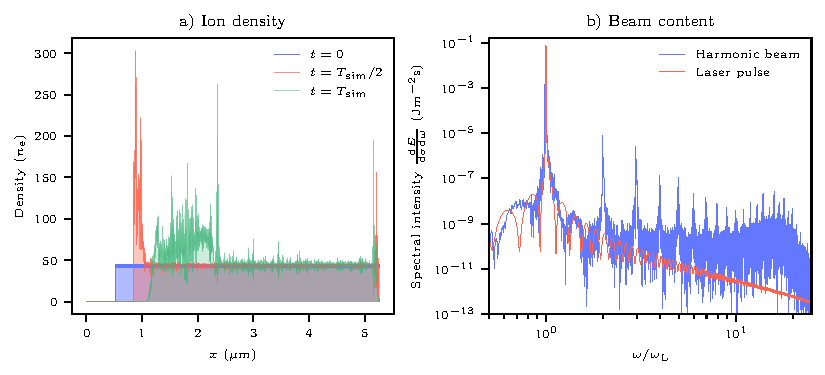
\includegraphics{figures/orion/orion_sim_figs}
	\caption[Typical 1D HHG Smilei simulation results]{\textbf{1D PIC simulation of the SP1 ORION beamline geometry at $\mathbf{a_0 = 7}$ interacting with a pre-ionised CVD target.} a) Ion density at initialisation ($t=0$), halfway ($t=T_\mathrm{sim}/2$) and at the simulation end ($t=T_\mathrm{sim}$) demonstrating hole boring. b) Absolute spectral intensity of the laser pulse and reflected harmonic beam obtained via Fourier transforms. The harmonic beam retains the laser pulse spectral width. Even harmonics are significantly suppressed at this polarisation. The large bump in the distribution around the 18\th\ harmonic is spuriously generated via numerical heating.}
	\label{fig:orionsimfigs}
\end{figure}
Figure \ref{fig:orionsimfigs}a illustrates how the ion density profile evolves via hole boring. While the density increases to several times its initial level near the plasma surface, this need not be accounted for in the hole boring calculation since these additional ions have already acquired the necessary momentum and are simply propagating inwards with the surface. Figure \ref{fig:orionsimfigs}b clearly shows the harmonic content of the specularly reflected beam with harmonics retaining the spectral shape of the incident beam. Even harmonics are significantly supressed relative to odd harmonics. The bump in the distribution around the 18\th\ harmonic is an entirely numerical effect, increasing the simulation resolution shifts the bump to the right. These simulations had a resolution of 128 cells per laser wavelength, following Edwards and Mikhailova one can only trust this distribution up to the 12\th\ harmonic, at which point the distribution begins to change its shape. Clearly energy conservation does not hold for this simulation, however it is still possible to extract $I_0$ if we make the reasonable assumption that Debye heating does not affect the HHG process and that the spectrum is simply the sum of the two contributions (justified by the observation of the continuation of harmonics over the bump in the distribution). Thus, $I_0$ can simply be extracted as the the peak intensity of the distribution corresponding to the intensity at $\omega/\omega_\mathrm{L} = 1$).

Figure \ref{fig:orioncombinedi0ds} compares the analytically calculated parameters with those extracted from the simulations demonstrating excellent agreement for the parameter space accessible with the ORION laser facility and for the assumptions made in the analysis.
\begin{figure}
	\centering
	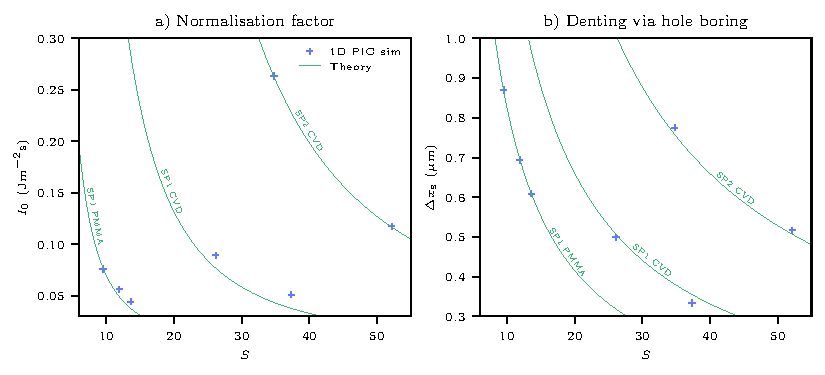
\includegraphics{figures/orion/orion_combined_I0_ds}
	\caption[Comparison between simulation and analytical predictions of hole boring and HHG normalisation factor.]{\textbf{Comparison between simulation and analytical predictions of hole boring and HHG normalisation factor in the ORION laser facility parameter space for CVD and PMMA targets.} a) The normalisation factor, $I_0$, where the spectral intensity, $I = I_0 n^{-p}$ for low order harmonics. b) The depth of hole boring compared to the initialised plasma surface. Note that the steep density gradient as visible in Figure \ref{fig:orionsimfigs}a ensures the surface position is well defined. Both parameters are expressed in the laboratory frame.}
	\label{fig:orioncombinedi0ds}
\end{figure}
% TODO get new plot of above with circ pol point included. Then write following
%Note that hole boring theory relies on the assumption of a quasi-static equilibrium. This is only true for a circularly polarised incident pulse.
The effect of numerical heating on the hole boring extent is evident in Figure X where the change in the surface position is plotted over time for the analytical calculation and PIC simulations with 2\nd\ and 4\th\ order shape function. 
\begin{figure}
	\centering
	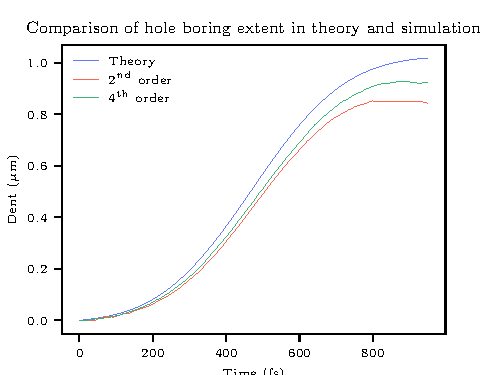
\includegraphics{figures/orion/orion_compare_ion_denting_to_theory}
	\caption[The effect of the PIC code particle shape function on numerical heating.]{\textbf{The effect of the PIC code particle shape function on numerical heating demonstrated via the extent of hole boring.} The deviation from the theoretical prediction increases with time, the error decreases for increasing order of the shape function.}
	\label{fig:orioncompareiondentingtotheory}
\end{figure}
The deviation from the theoretical prediction increases with time. Numerical heating leads to higher electron temperatures at the plasma surface and correspondingly a spurious preplasma expansion analogous to the prepulse preplasma expansion. This is why artificially increasing the plasma temperature to increase the Debye length and reduce numerical heating, while improving HHG accuracy, reduces hole boring accuracy since on sub-ps timescales, there is the potential for significant preplasma expansion.

The X-ray harmonic spectrum produced from a CVD target irradiated by an SP1 type laser pulse is resolved in Figure \ref{fig:orionxrayharmonics}.
\begin{figure}
	\centering
	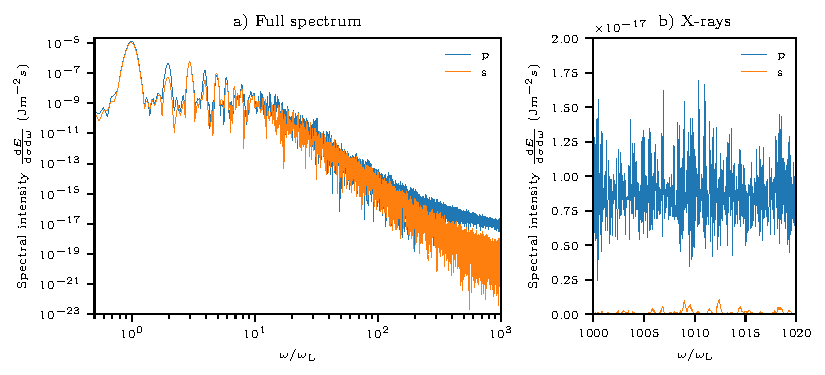
\includegraphics{figures/orion/orion_xray_harmonics}
	\caption[Reflected beam harmonic content up to the keV range in a high resolution 1D PIC simulation.]{\textbf{Reflected beam harmonic content up to the keV range in a high resolution 1D PIC simulation of a test pulse with SP1 ORION beam geometry incident on a CVD target.} The absolute spectral intensity is calculated from the Fourier transform of the reflected beam electric field. The s- and p-polarised components of the beam are analysed separately for both a) the full spectrum and b) the X-ray harmonics accessible with the OHREX quartz ($10\bar{1}1$) crystal.}
	\label{fig:orionxrayharmonics}
\end{figure}
The simulation has 16384 cells per laser wavelength, the minimum multiple of 2 required to resolve the harmonics accessed with the OHREX quartz crystals. It was necessary to use a short test laser pulse with a $5\lambda_\mathrm{L}$ FWHM. The simulation time before the peak of laser pulse was increased to reduce the error in the spectrum from unphysical hard cutoffs to the laser pulse profile. A steep preplasma scale length was applied to the plasma distribution of $0.04\lambda_\mathrm{L}$ to model the peak of the ORION pulse and suppress \ac{CWE}. At the X-ray intensities of Figure \ref{fig:orionxrayharmonics}b, no harmonic structure is visible, indeed for the non-optimal ORION target chamber geometry, harmonics begin to merge from around the 20\th . Note the s-polarised part of the reflected beam is over 50 times weaker than the p-polarised beam at the 1000\th\ harmonic.
It would be interesting to extract the reflected beam temporal profile after filtering of sub X-ray harmonics. This can be achieved by applying the inverse Fourier transform to the Fourier transformed temporal profile with the lower order harmonics removed. Unfortunately, beyond $n=50$, the contribution in the signal from noise prevented the structure from being observed. Figure \ref{fig:orionattosecondpulse} compares the reflected pulse structure to the reflected pulse structure with harmonics below $n = 50$ removed. 
\begin{figure}
	\centering
	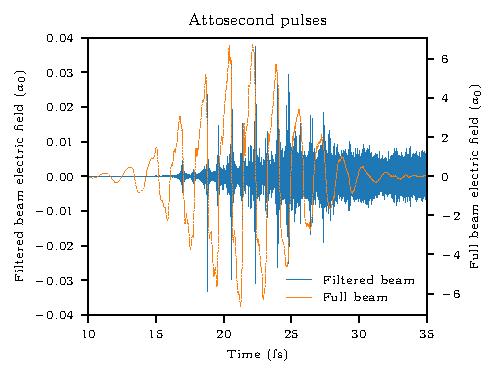
\includegraphics{figures/orion/orion_attosecond_pulse}
	\caption[Attosecond pulse train from the filtered reflected laser pulse.]{\textbf{Attosecond pulse train from the filtered reflected laser pulse.} The filtered beam contains only harmonics above $n = 50$.}
	\label{fig:orionattosecondpulse}
\end{figure}
The filtered beam consists of a series of attosecond pulses of radiation, the brightest pulse is of duration 30.3 as. Note that the intensity of the first few laser cycles is insufficient for the generation of harmonics above $n = 50$ and there is therefore no signal here, reducing the pulse train length.

% TODO Confident now that in the theory of ROM HHG for ORION parameters, there is one final consideration that cannot be observed in 1D. The SP1 beamline consists of two beamlets. Am I including this or no?
% TODO For this simulation, the Bouchard solver was applied.
% TODO A sharp density gradient was applied - return to this once reported on hydro sims.

\subsection{Hydrodynamic simulations of preplasma formation}\ref{sec:orion-hydro}
Following Dollar \textit{et al} \cite{dollarScalingHighorderHarmonic2013}, hydrodynamic simulations of the ORION laser systems were performed using HYADES to confirm the suitability of the contrast conditions.

To do: calculate intensity on target and PM. Discuss how there is potentially a range of laser intensities thus had `high' intensity and `low' intensity sims (state what these mean for the two beamlines.)
All simulations were performed with s- and p-polarisation.

Parameters:
1D planar geometry
Mesh of 511 evenly space points covering \qty{20}{\mu m} of the target (SiO2, PMMA, CVD, etc)
Equation of state data taken from the in built HYADES data tables. For low temperatures and pressures, the data for the minimum value in the tables is used, for temperatures and pressures above the highest value in the tables, the values are linearly extrapolated from the edge.
The local thermal equilibrium average atom model is used for ionisation. 
At low temperatures ($T < 0.15 eV$) the absoprtion and refractive indices are input.
The threshold for laser energy absorption is set to \qty{1e6}{ergs.cm^{-2}} = \qty{0.1}{W.cm^{-2}}.
Electrons and ions are initialised at a temperature \qty{1.551e-2}{eV}.




Results:
No pre-ionisation or preplasma formation was observed in the simulations of the high contrast SP1 laser pulse with any target materials. This is in stark contrast with the SP2 laser, in the absence of a PM, the preplasma expansion of the targets is huge. Necessitating the use of a PM and further HYADES simulations.
First, the interaction between the SP2 and SiO$_2$ plasma mirror was simulated. Note that it is not possible to model the AR coating in hydrodynamic codes, instead it was assumed that the thin coating has minimal impact on the interaction. No ionisation was observed from the high intensity laser prepulse starting from 10 ns out from the main pulse. Figure \ref{fig:orionpmirradiation} plots the interaction between a low intensity main pulse and the plasma mirror. 
\begin{figure}
	\centering
	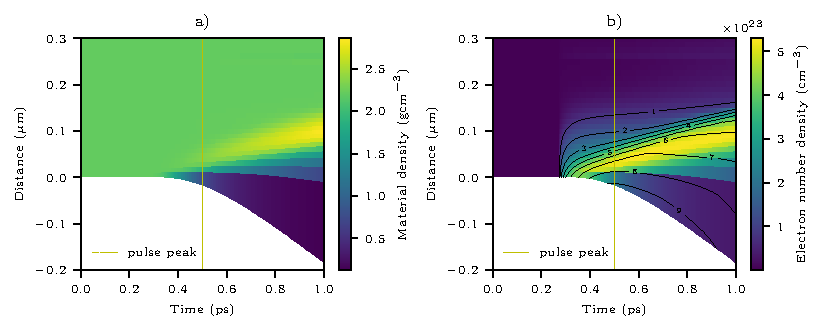
\includegraphics{figures/orion/orion_PM_irradiation}
	\caption[Silicon dioxide plasma mirror switch on from irradiation by the SP2 main pulse.]{\textbf{Silicon dioxide plasma mirror switch on from irradiation by the SP2 main pulseat \qty{45}{\degree} angle of incidence and p-polarisation.} The laser pulse travels in the $+\mathbf{\hat{x}}$-direction. The main pulse peak intensity is marked at 500 ps into the simulation. a) Material density as a function of time, a short preplasma is formed alongside hole boring. b) Electron number density as a function of time. The contours map the ionisation level.}
	\label{fig:orionpmirradiation}
\end{figure}
% TODO add comment about at this point jsut getting to that ionisation threshold?
Similar results were obtained for s- and p-polarisation. These simulations suggest ionisation begins at the start of the main pulse with some preplasma expansion but more significantly is the hole boring. Note that hole boring on the PM need not be accounted for since the spot size is significantly larger and therefore this change in surface curvature has minimal effect. The collisionless skin depth and plasma frequency can be calculated at each point in the plasma  via the electron densoty and the corresponding laser attenuation at each point as in Figure \ref{fig:orionpmreflection} at the peak of the main pulse.
\begin{figure}
	\centering
	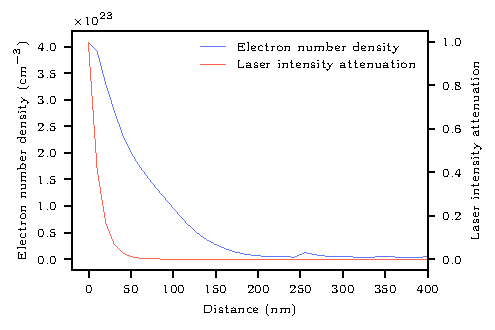
\includegraphics{figures/orion/orion_PM_reflection}
	\caption[The attenuation of the SP2 laser pulse as it propagates through a switched-on PM.]{\textbf{The attenuation of the SP2 laser pulse calculated as it propagates through a switched-on PM.}}
	\label{fig:orionpmreflection}
\end{figure}
The laser is rapidly attenuated and therefore `switched-on' despite not attaining total ionisation at the front surface (reducing its reflectivity).

Satisfied that the PM operates as anticipated, a parameter scan of the targets was then conducted. Figure \ref{fig:oriontargetpreplasma}a describes the typical evolution of target density with the application of the SP2 prepulse, in this case after that prepulse has been attenuated by a plasma mirror with a reflectivity of 0.004.
\begin{figure}
	\centering
	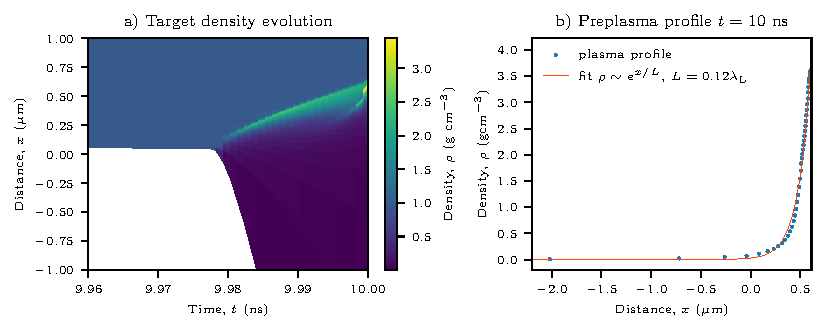
\includegraphics{figures/orion/orion_target_preplasma}
	\caption[Typical preplasma formation from the incidence of the ORION SP2 laser prepulse on a plastic target.]{\textbf{Typical preplasma formation from the p-polarised \qty{16}{\degree} angle of incidence of the ORION SP2 laser prepulse on an HDPE target.} In this simulation the laser is modelled from 10 ns before the main pulse with $a_0 = 30$ and attenuated by a PM of reflectivity 0.004. a) Typical preplasma expansion elucidated via target density. By the time of the main pulse, hole boring is dominant over plasma expansion. b) An exponetial fit ($\rho \sim e^{x/L}$) for the preplasma scale length, $L$, at the time of arrival of the main pulse. For this simulation the optimum fit is $L = 0.12 \lambda_\mathrm{L}$.}
	\label{fig:oriontargetpreplasma}
\end{figure}
By the time of the main pulse arrival in this simulation, hole boring has overtaken preplasma expansion. Figure \ref{fig:oriontargetpreplasma}b demonstrates the exponential fit to obtain the corresponding close to optimal preplasma scale length of $L = 0.12 \lambda_\mathrm{L}$ at the time of arrival of the SP2 main pulse.

Figure \ref{fig:orionscalelengthparameterscan} repeats the analysis of \ref{fig:oriontargetpreplasma} for a variety of target materials, reflectivities, polarisations and laser intensities.
\begin{figure}
	\centering
	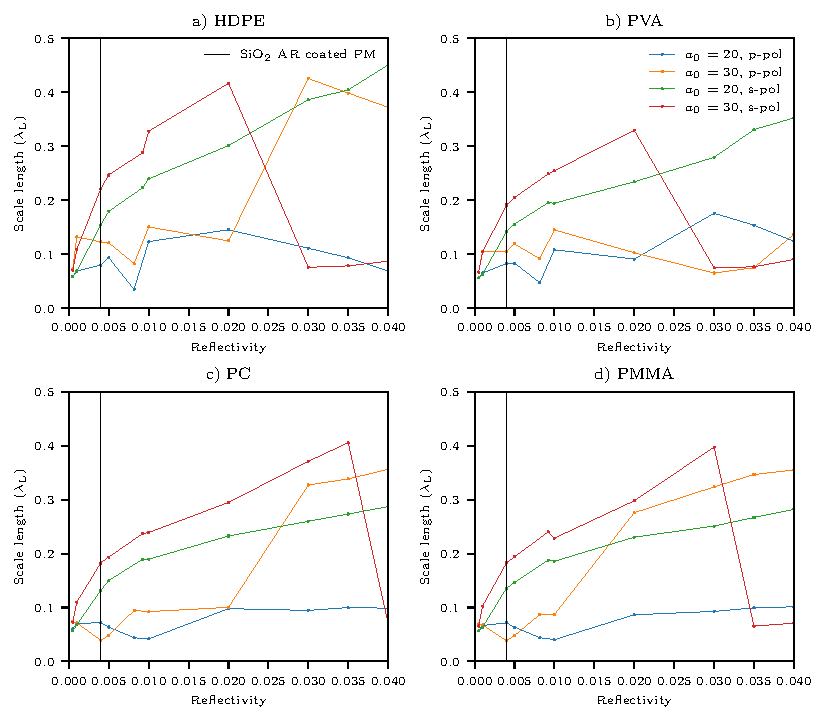
\includegraphics{figures/orion/orion_scale_length_parameter_scan}
	\caption[Preplasma scale length parameter scan.]{\textbf{Preplasma scale length parameter scan for a variety of plastic targets.} Target materials are a) HDPE, b) PVA, c) PC and d) PMMA. The dashed line highlights the reflectivity of the SiO$_2$ AR coated PM for the SP2 wavelength. Preplasma scale length remains small for the range of parameters explored.}
	\label{fig:orionscalelengthparameterscan}
\end{figure}
The s-polarised light simulations follow a clear trend: increasing incident laser energy leads to an increased scale length up to a transition point that will be determined by the point at which hole boring overcomes plasma expansion. This will depend on the interplay of target ion density, ionisation potential and heating. Interestingly, the trend is much less consistent for p-polarised light. It is known that heating increases for p-polarised light as there is now a component of the laser pulse electric field acting into the plasma, however, the crossing of the high and low intensities suggests a dynamic balance between hole boring and plasma heating. Regardless, the change in scale length is not significant at these PM reflectivities. Unfortunately, it was not possible to conduct a similar parameter scan for the CVD targets, it would appear that the EOS tables for such a target material are not suited for this interaction type, the two tables offered provided inconsistent and unphysical results with specific simulations crashing at random. However, one can assume that the preplasma scale lengths of irradiated CVD targets would be lower than those established in Figure \ref{fig:orionscalelengthparameterscan} due to the high damage threshold of the material. 

% TODO state somewhere that we can expect hole boring to establish itself at the time where the laser becomes relativistic since at this point electrons at the surface can be compressed and ions can follow.
%TODO ensure methodology clear

It is interesting to return to the question of temperature raised with regards to the initialisation of PIC code main pulse simulations as presented in Chapter \ref{ch:zvp}. Figure \ref{fig:oriontemperature} plots the plasma electron temperature from 40 ps before the main pulse arrives.
\begin{figure}
	\centering
	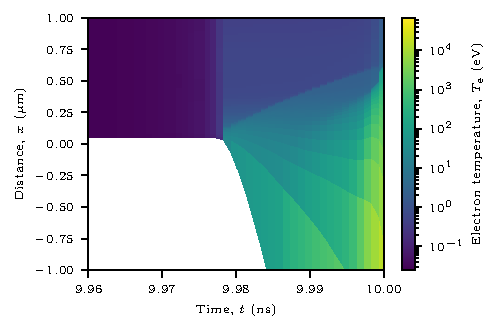
\includegraphics{figures/orion/orion_temperature}
	\caption[Typical electron temperature of a plastic target after irradiation by a petawatt class laser prepulse.]{\textbf{The typical electron temperature of a plastic target after irradiation by a petawatt class laser prepulse.} This is the same simulation as presented in Figure \ref{fig:oriontargetpreplasma}. Namely, an $a_0 = 30$ p-polarised laser pulse attenuated by a plasma mirror of reflectivity 0.004 incident on an HDPE target at \qty{16}{\degree}. The bulk and preplasma temperatures differ by multiple orders of magnitude.}
	\label{fig:oriontemperature}
\end{figure}
Once plasma expansion initiates the extent of heating rapidly diverges across the preplasma and bulk. Arguably it does not make sense to define a temperature for a system clearly not in equilibrium. Indeed, there is no standard practice and yet it can have significant effect such as has been seen in simulations on hole boring and \textbf{ paper on prepulses and cooler being better}. Clearly, plasma temperature will be highly sensitive to the precise experimental conditions. At the time of the main pulse arrival at plasma surface (as defined by the peak of the electron density distribution), the temperature is 112 eV, consistent with the value chosen for PIC simulations. Note that hydrodynamic codes would be unsuitable for the prediction of the plasma temperature increase from the main pulse interaction given the highly non-linear dynamics in this regime could not be accurately captured by such a code.

% TODO cite that paper that looks at prepulses and cooler prepulses being more suitable
% TODO (add to discussion of results) Then say unfortunately due to debris we were unable to do what we wanted with the IR laser. Comment about recompression with the SiN thin PM.
% TODO in intro explain local thermal equilibrium average atom model for ionisation.
% TODO look at book to get the absorption and refractive indices references.
% TODO Thingy about polarisation why we cant do combo. All performed in s and p and for the range of possible peak intensities. add to the intro to this section once I have found where I explained this in my notes
%TODO Still to do: chapter intro and theory, brems


To do tomorrow: final reuslts of this section, presentation, paper? then aim to finish theory by end of the conference?? then its jsut the experimental layout which should be quick enough

\section{\label{ch:3-sec:data_processing}Experimental data processing}
%TODO update plots in this section
\subsection{Image plate calibration}
Image plates (IPs) are reusable recording media that detect ionising radiation and are particularly suitable for the detection of X-rays produced in laser-plasma interactions. Their response is well understood and their sensitivities to a wide spectrum photon energies have been absolutely calibrated on the ORION facility \cite{meadowcroftEvaluationSensitivityFading2008}. Albeit for the FLA3000 scanner not the FLA7000 used in this experiment. However, the deviation in response is negligible for the photon energies measured. In this experiment the Fuji Biological Analysis System (BAS) TR-type IPs were used. They have a phosphor layer composed of $\mathrm{BaFBr_{0.085}I_{0.15}}$ with density \qty{2.61}{g.cm^{-3}} and thickness \qty{60}{\mu m} but no mylar layer. This makes them suitable for low energy X-ray detection. When scanned, the IP releases blue photons via photostimuated luminescence (PSL), which is then collected by a photomultiplier tube. The PSL value is generalised across scanner types from the measured `Grey' ($G$) value by
\begin{equation}
	\mathrm{PSL} = (0.23284G^2\times 10^{-9})\left(\frac{\Delta x}{100}\right)^2W\times 10^{-L/2},
\end{equation}
where $\Delta x$ is the scanner resolution (= \qty{25}{\mu m} in this experiment), $L$ is the latitude parameter, and
\begin{equation}
	W = 0.092906 + 1370.8e^{-0.014874V} +  654.24e^{-0.011026},
\end{equation}
where $V$ is the scanner voltage \cite{golovinCalibrationImagingPlates2021}.

IP photon sensitivity, $\psi$, the number of PSLs per incident photon, is dependent on photon energy. Meadowcroft \textit{et al} modelled this as,
\begin{equation}
	\psi_j = \eta(m_jh\nu + c_j),
\end{equation}
where $h\nu$ is the photon energy and $m_j$ and $c_j$ are linear fit parameters valid for specific energy ranges, $j$. For the Fuji BAS TR-type IP and for X-rays in the range 0-6.0 keV, $m_j = \qty{0.54\pm0.05}{mPSL.keV^{-1}}$ and $c_j = \qty{0.02\pm0.002}{mPSL}$. The IP absorption efficiency in mPSL per photon is
\begin{equation}
	\eta(h\nu,T_i,T_s) = \exp{(-n_\mathrm{i}\Phi_\mathrm{i} (h\nu)T_\mathrm{i})}[1-\exp{(-n_\mathrm{s}\Phi_\mathrm{s}(h\nu)T_\mathrm{s})}],
\end{equation}
where $n$ is the layer density, $\Phi(h\nu)$ is the total cross-section of the layer, $T$ the effective layer thickness, s and i correspond to the sensitive (phosphor) and insensitive (mylar) layers of the IP respectively \cite{izumiApplicationImagingPlates2006}. The first term is neglected in the absence of an insensitive (mylar) layer in TR-type IP. Below 50 keV, the dominant mode for X-ray absorption into the IP is the photo-electric effect, where
\begin{equation}
	\Phi_\mathrm{ph} \approx \num{3e12}\frac{Z^4}{(h\nu)^{3.5}}   
\end{equation}
and $Z$ is the atomic number \cite{fornalskiSimpleEmpiricalCorrection2018} and $\Phi_\mathrm{ph}$ is given in units of Barn per atom. At 2.4 keV, that corresponds to a sensitivity of 1.32 mPSL per incident photon.

It is generally inevitable that some time will elapse between laser shot and IP scan. For this experiment 30 minutes was typical, in which time some fading of the IP occurs that must be accounted for. IP fading can be modelled as an attenuation factor,
\begin{equation}\label{eq:orion.Ft}
	F(t) = A\exp{(-t/\tau)} + B,
\end{equation}
where $t$ is the time between shot and scan and $A$, $\tau$ and $B$ are found from fits to experimental data. A key aspect of the exponential decay is that the attenuation depends only on the signal at that moment in time and not the initial conditions. This has been shown to be true in experiment \cite{meadowcroftEvaluationSensitivityFading2008}.

At \qty{20}{\degree C} at the ORION facility \textit{Meadowcroft et al} \cite{meadowcroftEvaluationSensitivityFading2008} determined that for the Fuji BAS TR-type IP, the optimum fit for the parameters of Equation \ref{eq:orion.Ft} is $A = \num{0.347\pm0.022}$, $B = \num{0.693\pm0.011}$ and $\tau = \qty{35.5\pm5.3}{minutes}$. Therefore at 30 minutes, $F(t) = 0.84$.

In summary, the number of PSL measured on an IP can be converted to an incident number of photons via
\begin{equation}
	N(h\nu) = \frac{\mathrm{PSL}}{F(t)}\frac{10^3}{\psi(h\nu)} = P(h\nu) \mathrm{PSL}.
\end{equation}

\subsection{OHREX calibration}
% TODO Reword note on illuminating crystal once I have written up about hole boring.
The Orion High REsolution X-ray (OHREX) spectrometer, housed on the ORION laser target chamber outer wall, utilises a spherically bent crystal geometry to spatially focus and spectrally analyse photons from the target chamber \cite{beiersdorferLineshapeSpectroscopyVery2016} with a high signal-to-noise ratio. The measured signal has been absolutely calibrated for a range of energies using a variety of crystals \cite{macdonaldAbsoluteThroughputCalibration2021}. The OHREX spectrometer can hold two crystals at a time. At each crystal's spatial focal plane a two-dimensional image is formed, one dimension is spatial, the other spectral. The energy range accessed by a given crystal is determined by the crystal rotation but all OHREX crystals are designed for operation at a nominal central Bragg angle of $\theta_\mathrm{B} = 51.3$\degree with the corresponding wavelength determined from Bragg's Law, $n\lambda = 2d\sin\theta_\mathrm{B}$, for the appropriate crystal plane. The range around that central photon energy is determined by the crystal width in the spectral dimension.

MacDonald \textit{et al} determined a quadratic fit for each crystal's dispersion relation to connect position along the image to photon energy \cite{macdonaldAbsoluteThroughputCalibration2021}. Unfortunately in this experiment, the image lengths varied from those in the previous experiment, a likely consequence of slight defocusing of the optic. Note that the OHREX geometry is designed such that precise focus is not necessary to achieve good results \cite{beiersdorferLineshapeSpectroscopyVery2016}.

Instead, a simple linear dispersion relation based on the known maximum and minimum energies accessed by the crystal was applied across the crystal images, a reasonable approximation to the dispersion relation determined by MacDonald \textit{et al} \cite{macdonaldAbsoluteThroughputCalibration2021} (the quadratic correction is small). The energy ranges for the three lowest energy OHREX crystals are given in table \ref{tab:dispersion}.
\begin{table}
	\centering
\begin{tabular}{ccc}
	\hline \hline
	Crystal               & Range, $n=1$ (eV) & Range, $n=2$ (eV) \\ \hline
	KAP (100)             & 585-625          & 1170-1245        \\
	Quartz ($10\bar{1}0$) & 1830-1950        & 3660-3900        \\
	Quartz ($10\bar{1}1$) & 2330-2480        & 4660-4960  \\     \hline \hline
\end{tabular}
	\caption{\label{tab:dispersion} Photon energy ranges captured by the three lowest energy OHREX crystals when operating at their nominal central Bragg angle of 51.3\degree for first and second diffraction orders, $n$.}
\end{table}

Provided full illumination of the \qty{6}{cm} $\times$ \qty{4}{cm} crystal, the spatial dimension can be safely integrated over to calculate the measured signal, $M(h\nu)$ in \unit{J.mm^{-1}} and remove uncertainty from the IP drifting from the ideal focal plane. (In this experiment we assume that the harmonic beam width at the crystal position is larger than the size of the crystal, a reasonable assumption since beam divergence $\approx$ \qty{10}{\degree} and the \qty{6}{cm} x \qty{4}{cm} crystal sits \qty{2.4}{m} from the target.). This corresponds to a source spetral intensity incident on the crystal $S(h\nu)$ measured in \unit{J.keV^{-1}.sr^{-1}} via the spectrometer response, $G(h\nu)$, explicitly,
\begin{equation}
	M(h\nu) = S(h\nu)G(h\nu).
\end{equation}
The absolute throughput of the crystals was measured by MacDonald \textit{et al} in a previous ORION experiment and fit parameters for 
\begin{equation}
	G(h\nu) = A(h\nu)^2 + B(h\nu) + C,
\end{equation}
where $(h\nu)$ is the photon energy measured in eV, determined for both p- and s-polarised incident light and for first and second diffraction orders \cite{macdonaldAbsoluteThroughputCalibration2021}. The parameters for the lowest few energy crystals are presents in Table \ref{tab:orion_OHREX}.
\begin{table}
\centering
\begin{tabular}{cccccc}
	\hline \hline
	Crystal               & Order & Polarisation & $A$            & $B$             & $C$            \\
	\hline
	KAP             & 1     & s            & \num{1.72e-15} & \num{-4.69e-12} & \num{2.89e-9}  \\
	(100) &       & p            & \num{1.40e-14} & \num{-1.74e-11} & \num{5.42e-9}  \\
	& 2     & s            & \num{3.64e-16} & \num{-9.64e-13} & \num{6.95e-10} \\
	&       & p            & \num{5.03e-10} & \num{8.09e-13}  & \num{5.03e-10} \\
	Quartz  & 1     & s            & $\cdots$       & $\cdots$        & $\cdots$       \\
	  ($10\bar{1}0$)&     & p            & $\cdots$       & $\cdots$        & $\cdots$       \\
	& 2     & s            & \num{4.50e-15} & \num{-3.40e-11} & \num{6.52e-8}  \\
	&       & p            & \num{1.13e-15} & \num{-8.86e-12} & \num{1.73e-8}  \\
	Quartz  & 1     & s            & \num{1.00e-16} & \num{-1.74e-12} & \num{4.93e-9}  \\
	  ($10\bar{1}1$)&     & p            & \num{2.78e-15} & \num{-1.41e-11} & \num{1.79e-8}  \\
	& 2     & s            & \num{4.70e-16} & \num{-4.50e-12} & \num{1.11e-8}  \\
	&       & p            & \num{2.10e-16} & \num{2.11e-12}  & \num{5.30e-9}  \\
	\hline \hline
\end{tabular}
\caption{Sensitivity fit parameters as a function of photon energy, $h\nu$ in electron-volts ($G(h\nu) = A(h\nu)^2 + B(h\nu) + C$) for the three lowest energy OHREX crystals for p- and s-polarised incident photons and first and second diffraction orders \cite{macdonaldAbsoluteThroughputCalibration2021}. Note that no data is available for the first order of the quartz ($10\bar{1}0$) crystal.}
\label{tab:orion_OHREX}
\end{table}
There is unfortunately no spectrometer response data for the $10\bar{1}0$ crystal to first order due to the Si K edge sitting within the energy range and the dramatic effect this has on absorption in its vicinity \cite{hellCalibrationOHREXHighresolution2016}.


The OHREX is equipped with a \qty{50}{\mu m} Beryllium filter to protect the crystals. The corresponding signal attenuation can be calculated using X-ray transmission data \cite{henkeXRayInteractionsPhotoabsorption1993a}.

\subsection{Extracting the data}
The quartz OHREX crystals $10\bar{1}0$ and $10\bar{1}1$ were fielded on the experiment. Crystal images were recorded with BasTR2040 Fuji Image Plate. A typical shot image scanned with the FLA7000 scanner and converted to photostimulated luminescence units (PSLs) is given in Figure \ref{fig:orionohrexshot28psl}.
%todo point out both crystal images and label them
\begin{figure}
	\centering
	\includegraphics[width=0.5\linewidth]{figures/orion/orion_OHREX_shot28_psl}
	\caption[Unprocessed IP from ORION experiment]{Unprocessed shot data from a FLA7000 scanned image plate converted to PSLs. The image plate and two crystal images are clearly visible.}
	\label{fig:orionohrexshot28psl}
\end{figure}
The average background signal was subtracted. The $x$- and $y$-axes were converted from pixels to to mm using the scanner resolution, (\qty{25}{\mu m.px^{-1}}) and then energies using the appropriate dispersion relations. The data was then integrated over $y$ to obtain the intensity in units of \unit{PSL.mm^{-1}} across each crystal image. Then the corresponding source signal is
\begin{equation}
	S(h\nu)[\unit{J.keV^{-1}.sr^{-1}}] = \frac{d\mathrm{PSL}}{dx}\frac{P(h\nu)}{G(h\nu)}h\nu,
\end{equation}
which can then be converted to a measured spectral intensity per harmonic at distance $r=1$ from the source, ready to be directly compared to the theory,
\begin{equation}
	I^\mathrm{meas}_\mathrm{n}|_{(r = \qty{1}{m})} = S(h\nu)\frac{dh\nu(keV)}{dn}.
\end{equation}

No sensitivity data is available for the $10\bar{1}0$ quartz crystal, instead this lower energy crystal was fielded to attempt resolving of the X-ray harmonics. At the experiment planning stage it was unknown if this would be possible. Now that the simulations have been performed, we know that the non-optimal ORION target chamber geometry leads to merging of the harmonics even before the water window at 282 eV. This is consistent with the findings, Figure \ref{fig:orionq1010} is a typical integrated signal in \unit{PSL.mm} and the corresponding Fourier transform for the quartz ($10\bar{1}0$) crystal image.
\begin{figure}
	\centering
	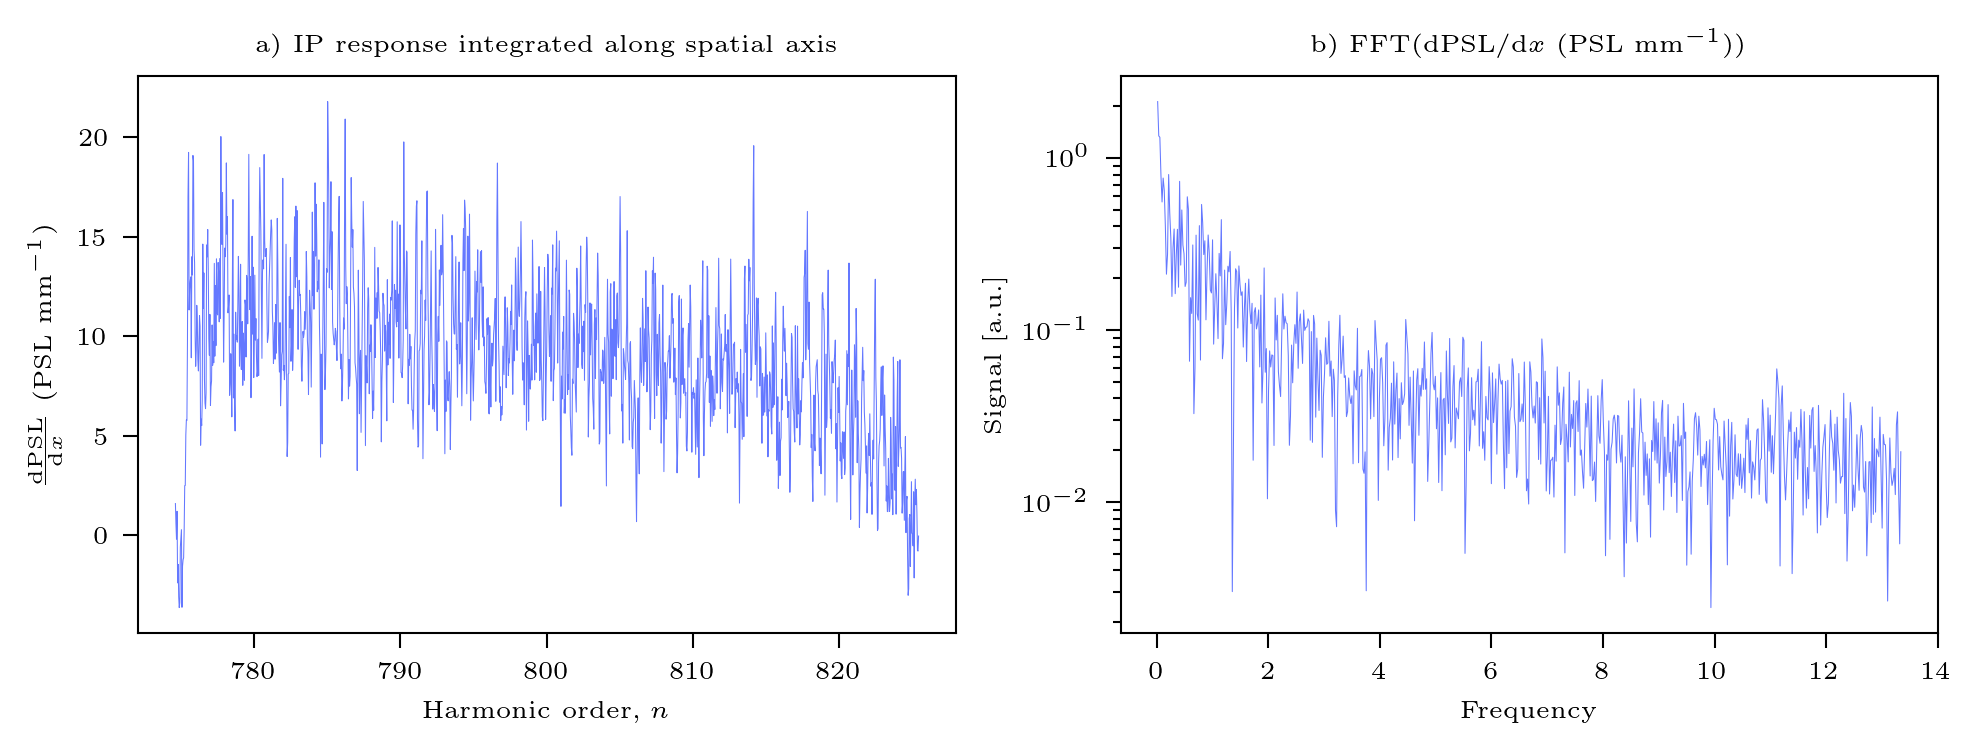
\includegraphics[width=1\linewidth]{figures/orion/orion_q1010}
	\caption[Typical ORION experiment uncalibrated IP response quartz ($10\bar{1}0$) crystal and Fourier transform]{\textbf{Typical (SP1, PMMA) uncalibrated shot data for the quartz ($10\bar{1}0$) image} a) IP spatial axis integrated signal with dispersion axis. b) Fourier transform of a) with no evidence of harmonics.}
	\label{fig:orionq1010}
\end{figure}

\subsubsection{Calibration and polarisation}
% TODO reference simulation figure that shows only p pol light reflected.
% TODO write up the OHREX polarisation stuff
% TODO put efficiency of only p pol reflected into the theory prediction, I think at this moment I am coming at it from the experiment side which is wrong.
% TODO add in polarisations of SP1 and SP2 for the OHREX angles out of the plane.
The choice of the spectrometer response function, $G(h\nu)$, is non-trivial. One must firstly be assured that the second order contribution is small relative to the first, true for this source spectrum. And also think carefully about the anticipated polarisation in the OHREX interaction plane. The OHREX response to p-polarised light is approximately an order of magnitude lower than for s-polarised light. From Figure X we are assured that only the p-polarised (with respect to the target interaction plane) X-rays are specularly reflected to the OHREX. Corresponding polarisation out of the OHREX interaction plane is calculated in the Appendix. The polarisation of the HHG beam relative to the OHREX plane of incidence and reflection is \qty{10.5}{\degree} out of the plane. Unlike for the RPM interaction, the OHREX crystal reflection is an entirely linear process and it is therefore acceptable to decompose the laser pulse into its constituents, explicitly, the field incident on the crystal is
\begin{equation}
	\mathbf{E_\mathrm{O}} = \mathbf{E}_\mathrm{O,\, s} + \mathbf{E}_\mathrm{O,\, p}.
\end{equation}
After interaction with the crystal the field is
\begin{equation}
	\mathbf{E}_\mathrm{detector} = \alpha_\mathrm{s}(h\nu)\mathbf{E}_\mathrm{O,\, s} + \alpha_\mathrm{p}(h\nu)\mathbf{E}_\mathrm{O,\, p},
\end{equation}
where $\alpha_i(h\nu)$ is the energy dependent $(h\nu)$ amplitude sensitivity of the reflection for s- and p-polarised respectively. Since the two polarisations are orthogonal, the intensity is
\begin{equation}
	I = \alpha^2_\mathrm{s}(h\nu)|\mathbf{E}_\mathrm{O,\, s}|^2 + \alpha^2_\mathrm{p}(h\nu)|\mathbf{E}_\mathrm{O,\, p}|^2.
\end{equation}
Noting that $\alpha^2_i(h\nu)$ are the calibration factors, $G_i(h\nu)$, and that
\begin{equation}
	|\mathbf{E}_\mathrm{O,\, s}| = |\mathbf{E_\mathrm{O}}|\sin\phi
\end{equation}
and
\begin{equation}
	|\mathbf{E}_\mathrm{O,\, p}| = |\mathbf{E_\mathrm{O}}|\cos\phi,
\end{equation}
where $\phi$ is the angle out of the interaction plane,
\begin{equation}
	I_\mathrm{detector} = (G_\mathrm{s}(h\nu)\sin^2\phi + G_\mathrm{p}(h\nu)\cos^2\phi)|\mathbf{E_\mathrm{O}}|^2 = F(h\nu)|\mathbf{E_\mathrm{O}}|^2,
\end{equation}
where $F(h\nu) =  (G_\mathrm{s}(h\nu)\sin^2\phi + G_\mathrm{p}(h\nu)\cos^2\phi$ is the energy dependent calibration factor for this OHREX orientation.

\section{Experimental results}

Figure \ref{fig:orionq1011} is a typical calibrated signal from the quartz ($10\bar{1}1$) crystal, ready for comparison to the theoretical prediction.
\begin{figure}
	\centering
	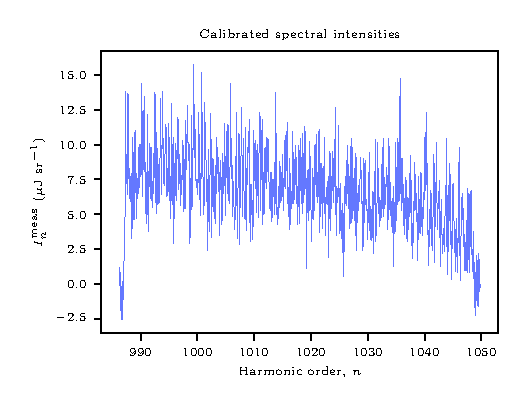
\includegraphics[width=0.7\linewidth]{figures/orion/orion_q1011}
	\caption[Typical ORION experiment calibrated IP response for the quartz ($10\bar{1}1$) crystal.]{Typical (SP1, PMMA) ORION experiment calibrated IP response for the quartz ($10\bar{1}1$) crystal.}
	\label{fig:orionq1011}
\end{figure}
For each shot the mean signal across the dispersion axis was calculated and the errors from statistics, the fade time (11 \%), the IP sensitivity (1.5 \%), the dispersion axis (2.9 \%) and the OHREX crystal reflectivity (11 \%) accounted for.
% TODO Shots were also taken through the OHREX port, we had hoped to capture the beam divergence however, the beam was larger than initially expected and we were unable to distinguish much. Mention saturation.

As demonstrated in Section \ref{ch:3-sec:theory}, the intensity of X-ray harmonics is highly sensitive to the intensity of individual pulse cycles due to the proximity of the measurement to the exponential roll off in the spectrum. However, even neglecting the shot-to-shot variation, it is not possible to know the precise sub-cycle spatio-temporal struture of a petawatt-class laser pulse. Indeed, the simple measurement of the peak intensity of such a pulse remains an open problem \cite{perevalovLaserPeelerRegime2023,ouatuIonizationStatesMultipetawatt2022}. Instead we must rely on our assumptions and approximations, that is that the SP1 and SP2 beamlines can be adequately described by spatial Gaussians and temporal sech$^2$ and sech profiles respectively, and that the duration and energy are well defined. The tight focused laser spot is subject to jitter on a shot-to-shot basis. This was routinely monitored via a KBRXM diagnostic that measures X-ray emission from the target. The spot measured by this diagnostic will always be larger than the actual laser pulse focal spot due to the energy transport of electrons moving away from the interaction area. This upper limit on laser pulse spot size corresponds to a lower limit on laser pulse intensity and therefore also of HHG efficiency. Figure \ref{fig:orionintensitycurves} plots HHG spectral intensity curves for the quartz ($10\bar{1}1$) crystal central energy as a function of laser spot size for the targets and laser pulse configurations explored in the experiment. 
\begin{figure}
	\centering
	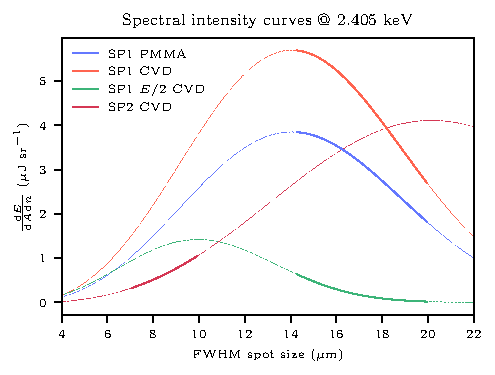
\includegraphics{figures/orion/orion_intensity_curves}
	\caption[Dependence of the harmonic beam spectral intensity on laser spot size at 2.405 keV.]{\textbf{Dependence of the harmonic beam spectral intensity on laser spot size at 2.405 keV.} Targets and beamlines relevant to the experiment are plotted. The half energy single beamlet SP1 laser is demarcated by $E/2$. The thick lines indicate likely values for the laser spot sizes in this experiment. The SP1 harmonic beams are strongly affected by the exponential roll off unlike the SP2 beamline.}
	\label{fig:orionintensitycurves}
\end{figure}
The thick lines range from the uppper limits of spot size as measured by the KBRXM diagnostic to the spot area being halved. The spectral intensity of the harmonic beam from the SP1 beamline sits in a delicate balance between beam divergence via hole boring and the exponential roll off. Note that only the roll off leads to a reduction in the total energy contained within the harmonic beam. The strong non-linearity of the interaction leads to the single beamlet SP1 beamline producing a harmonic beam over 6 times weaker than the double beamlet configuration. Interestingly, the higher intensity of the SP2 beamline leads to a greater divergence and a lower spectral intensity of the harmonic beam than for the SP1 laser pulse.

Figure \ref{fig:orionexperimentresults} plots the experimental results with comparison to theory and simulation. 
\begin{figure}
	\centering
	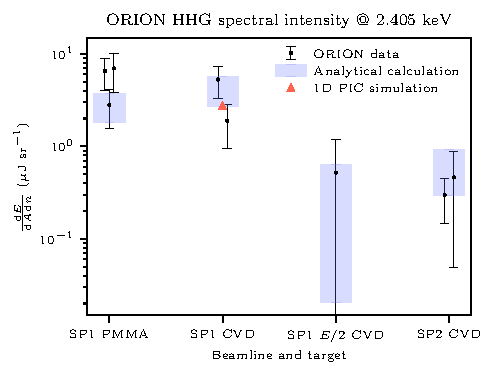
\includegraphics{figures/orion/orion_experiment_results}
	\caption[X-ray harmonic intensities measured on the ORION experiment compared to theory and simulation.]{\textbf{X-ray harmonic spectral intensities at 2.405 keV measured on the ORION experiment compared to theory and simulation.} The analytical calculation corresponds to the thick lines marked in Figure \ref{fig:orionintensitycurves}. The 1D PIC simulation result is derived from Figure \ref{fig:orionxrayharmonics} and scaled to the ORION laser pulse duration.}
	\label{fig:orionexperimentresults}
\end{figure}
Experimental data points are consistent within their errors with one another, the theory and the simulation, albeit with large uncertainties with such a low shot number. It is highly significant that the SP2 beamline is on average almost 6 times brighter than the SP1 beamline despite the greater energy content and greater component of the laser pulse electric field directed into the plasma for the SP2 beamline while the single beamlet shot is over 7 times weaker in intensity compared to the mean intensity of the full SP2 beamline. These highly non-linear (with respect to energy) scalings are consistent with HHG theory but cannot be understood as originating from bremmstrahlung lending huge credibility to these results. Bremsstrahlung emission scales sub-linearly with temperature and temperature scales sub-linearly with energy on target. The total energy is well-constrained and this is far more relevant for Bremsstrahlung than the uncertain intensity (dependent on the variable spot size). Thus, at best case scenario one could anticipate twice the intensity being observed for the double beamlet SP2 compared to the single.





Bremsstrahlung emission from steep density profile low-Z solid density targets irradiated by relativistic laser pulses remains an area of active research with experiments to explore this in the planning stages at the University of York. However, provided a few assumptions it is possible to derive approximate best case scenario scalings of spectral intensity with incident energy. First, assume that energy absorption into the plasma target does not increase with increasing energy. From Equation
% TODO add derivation of plasma temperature from start of Chen to intro then reference here
the plasma temperature scales linearly with the incident energy. Now, assuming the target can be treated as a radiating black body, Equation 
% TODO add note on black body and and reference spectral radiance here
increases most rapidly with temperature when $h\nu \ll k_\mathrm{B}T$ at which point the spectral radiance scales linearly with temperature. Thus, at best case we could expect a linear increase in the spectral intensity measured from the double beamlet compared to the single if that signal originated from Bremsstrahlung emission. Note further that this scaling depends not on the incident intensity but only on the incident energy which is a well-constrained quantity on ORION, \textit{i.e.} we do not anticipate significant shot-to-shot variation.

The above discussion relied on the assumptions of equilibrium and a black-body radiation spectrum.
While this is valid for the long radiating period after the interaction, in much of this thesis, emphasis has been placed on the non-equilibrium state of the interaction itself. There are two species of relevance during this time: the hot electrons around the front surface directly heated by the laser pulse and prepulse, and the hot electrons that are reflected specularly and are responsible for the HHG. In \cite{zulickHighResolutionBremsstrahlung2013}, bremsstrahlung of these species are measured experimentally for a 30 fs laser pulse and $a_0$ = 2.8. As the populations of each of these species are so small, the peak contribution to the photon spectrum is many orders of magnitude smaller than that of the experimental signal and can therefore be neglected.
% TODO check in the above that they used a circualrly pol pulse so that HHG would be supperssed?

These findings are highly significant. 
Then write up the new peak intensity and the efficiencies.
Comment on flying focus

% TODO reference beam on Vulcan, it was 2 orders of magnitude above background from brems, thus we can assume above brems even if beam more divergence than ORION (would need to be 10 times as divegent)

% TODO Additional things: approximate reflectivity of the plasma mirror at switch on, merging of harmonics at the X-ray regime
% TODO describe KBRXM diagnostic 
% TODO Discuss mirrored targets and brems emission.

% Note that if you replace the spatial gaussian with a sinc^2 profile with the same FWHM, they look almost identical to exponential. The spatial integral is approx 1.06 times larger thus minimal impact on the profile
 